\documentclass[twoside]{book}

% Packages required by doxygen
\usepackage{calc}
\usepackage{doxygen}
\usepackage{graphicx}
\usepackage[utf8]{inputenc}
\usepackage{makeidx}
\usepackage{multicol}
\usepackage{multirow}
\usepackage{textcomp}
\usepackage[table]{xcolor}

% Font selection
\usepackage[T1]{fontenc}
\usepackage{mathptmx}
\usepackage[scaled=.90]{helvet}
\usepackage{courier}
\usepackage{amssymb}
\usepackage{sectsty}
\renewcommand{\familydefault}{\sfdefault}
\allsectionsfont{%
  \fontseries{bc}\selectfont%
  \color{darkgray}%
}
\renewcommand{\DoxyLabelFont}{%
  \fontseries{bc}\selectfont%
  \color{darkgray}%
}

% Page & text layout
\usepackage{geometry}
\geometry{%
  a4paper,%
  top=2.5cm,%
  bottom=2.5cm,%
  left=2.5cm,%
  right=2.5cm%
}
\tolerance=750
\hfuzz=15pt
\hbadness=750
\setlength{\emergencystretch}{15pt}
\setlength{\parindent}{0cm}
\setlength{\parskip}{0.2cm}
\makeatletter
\renewcommand{\paragraph}{%
  \@startsection{paragraph}{4}{0ex}{-1.0ex}{1.0ex}{%
    \normalfont\normalsize\bfseries\SS@parafont%
  }%
}
\renewcommand{\subparagraph}{%
  \@startsection{subparagraph}{5}{0ex}{-1.0ex}{1.0ex}{%
    \normalfont\normalsize\bfseries\SS@subparafont%
  }%
}
\makeatother

% Headers & footers
\usepackage{fancyhdr}
\pagestyle{fancyplain}
\fancyhead[LE]{\fancyplain{}{\bfseries\thepage}}
\fancyhead[CE]{\fancyplain{}{}}
\fancyhead[RE]{\fancyplain{}{\bfseries\leftmark}}
\fancyhead[LO]{\fancyplain{}{\bfseries\rightmark}}
\fancyhead[CO]{\fancyplain{}{}}
\fancyhead[RO]{\fancyplain{}{\bfseries\thepage}}
\fancyfoot[LE]{\fancyplain{}{}}
\fancyfoot[CE]{\fancyplain{}{}}
\fancyfoot[RE]{\fancyplain{}{\bfseries\scriptsize Generated on Sat Nov 16 2013 12\-:34\-:17 for Small\-World by Doxygen }}
\fancyfoot[LO]{\fancyplain{}{\bfseries\scriptsize Generated on Sat Nov 16 2013 12\-:34\-:17 for Small\-World by Doxygen }}
\fancyfoot[CO]{\fancyplain{}{}}
\fancyfoot[RO]{\fancyplain{}{}}
\renewcommand{\footrulewidth}{0.4pt}
\renewcommand{\chaptermark}[1]{%
  \markboth{#1}{}%
}
\renewcommand{\sectionmark}[1]{%
  \markright{\thesection\ #1}%
}

% Indices & bibliography
\usepackage{natbib}
\usepackage[titles]{tocloft}
\setcounter{tocdepth}{3}
\setcounter{secnumdepth}{5}
\makeindex

% Hyperlinks (required, but should be loaded last)
\usepackage{ifpdf}
\ifpdf
  \usepackage[pdftex,pagebackref=true]{hyperref}
\else
  \usepackage[ps2pdf,pagebackref=true]{hyperref}
\fi
\hypersetup{%
  colorlinks=true,%
  linkcolor=blue,%
  citecolor=blue,%
  unicode%
}

% Custom commands
\newcommand{\clearemptydoublepage}{%
  \newpage{\pagestyle{empty}\cleardoublepage}%
}


%===== C O N T E N T S =====

\begin{document}

% Titlepage & ToC
\hypersetup{pageanchor=false}
\pagenumbering{roman}
\begin{titlepage}
\vspace*{7cm}
\begin{center}%
{\Large Small\-World }\\
\vspace*{1cm}
{\large Generated by Doxygen 1.8.5}\\
\vspace*{0.5cm}
{\small Sat Nov 16 2013 12:34:17}\\
\end{center}
\end{titlepage}
\clearemptydoublepage
\tableofcontents
\clearemptydoublepage
\pagenumbering{arabic}
\hypersetup{pageanchor=true}

%--- Begin generated contents ---
\chapter{Small\-World}
\label{md__c_1__users_damienc__documents__git_hub__small_world__r_e_a_d_m_e}
\hypertarget{md__c_1__users_damienc__documents__git_hub__small_world__r_e_a_d_m_e}{}
Jeu Small\-World, dans le cadre d'un projet scolaire. 
\chapter{Namespace Index}
\section{Packages}
Here are the packages with brief descriptions (if available)\-:\begin{DoxyCompactList}
\item\contentsline{section}{\hyperlink{namespace_small_world}{Small\-World} }{\pageref{namespace_small_world}}{}
\item\contentsline{section}{\hyperlink{namespace_small_world_1_1_properties}{Small\-World.\-Properties} }{\pageref{namespace_small_world_1_1_properties}}{}
\end{DoxyCompactList}

\chapter{Hierarchical Index}
\section{Class Hierarchy}
This inheritance list is sorted roughly, but not completely, alphabetically\-:\begin{DoxyCompactList}
\item \contentsline{section}{Small\-World.\-Constantes}{\pageref{class_small_world_1_1_constantes}}{}
\item \contentsline{section}{Small\-World.\-Inter\-Carte}{\pageref{interface_small_world_1_1_inter_carte}}{}
\begin{DoxyCompactList}
\item \contentsline{section}{Small\-World.\-Carte}{\pageref{class_small_world_1_1_carte}}{}
\end{DoxyCompactList}
\item \contentsline{section}{Small\-World.\-Inter\-Case}{\pageref{interface_small_world_1_1_inter_case}}{}
\begin{DoxyCompactList}
\item \contentsline{section}{Small\-World.\-Case}{\pageref{class_small_world_1_1_case}}{}
\begin{DoxyCompactList}
\item \contentsline{section}{Small\-World.\-Desert}{\pageref{class_small_world_1_1_desert}}{}
\item \contentsline{section}{Small\-World.\-Eau}{\pageref{class_small_world_1_1_eau}}{}
\item \contentsline{section}{Small\-World.\-Foret}{\pageref{class_small_world_1_1_foret}}{}
\item \contentsline{section}{Small\-World.\-Montagne}{\pageref{class_small_world_1_1_montagne}}{}
\item \contentsline{section}{Small\-World.\-Plaine}{\pageref{class_small_world_1_1_plaine}}{}
\end{DoxyCompactList}
\item \contentsline{section}{Small\-World.\-Inter\-Desert}{\pageref{interface_small_world_1_1_inter_desert}}{}
\begin{DoxyCompactList}
\item \contentsline{section}{Small\-World.\-Desert}{\pageref{class_small_world_1_1_desert}}{}
\end{DoxyCompactList}
\item \contentsline{section}{Small\-World.\-Inter\-Eau}{\pageref{interface_small_world_1_1_inter_eau}}{}
\begin{DoxyCompactList}
\item \contentsline{section}{Small\-World.\-Eau}{\pageref{class_small_world_1_1_eau}}{}
\end{DoxyCompactList}
\item \contentsline{section}{Small\-World.\-Inter\-Foret}{\pageref{interface_small_world_1_1_inter_foret}}{}
\begin{DoxyCompactList}
\item \contentsline{section}{Small\-World.\-Foret}{\pageref{class_small_world_1_1_foret}}{}
\end{DoxyCompactList}
\item \contentsline{section}{Small\-World.\-Inter\-Montagne}{\pageref{interface_small_world_1_1_inter_montagne}}{}
\begin{DoxyCompactList}
\item \contentsline{section}{Small\-World.\-Montagne}{\pageref{class_small_world_1_1_montagne}}{}
\end{DoxyCompactList}
\item \contentsline{section}{Small\-World.\-Inter\-Plaine}{\pageref{interface_small_world_1_1_inter_plaine}}{}
\begin{DoxyCompactList}
\item \contentsline{section}{Small\-World.\-Plaine}{\pageref{class_small_world_1_1_plaine}}{}
\end{DoxyCompactList}
\end{DoxyCompactList}
\item \contentsline{section}{Inter\-Coordonnees}{\pageref{interface_inter_coordonnees}}{}
\item \contentsline{section}{Small\-World.\-Inter\-Cordonnees}{\pageref{interface_small_world_1_1_inter_cordonnees}}{}
\begin{DoxyCompactList}
\item \contentsline{section}{Small\-World.\-Coordonnees}{\pageref{class_small_world_1_1_coordonnees}}{}
\end{DoxyCompactList}
\item \contentsline{section}{Small\-World.\-Inter\-Createur\-Partie}{\pageref{interface_small_world_1_1_inter_createur_partie}}{}
\begin{DoxyCompactList}
\item \contentsline{section}{Small\-World.\-Createur\-Partie}{\pageref{class_small_world_1_1_createur_partie}}{}
\end{DoxyCompactList}
\item \contentsline{section}{Small\-World.\-Inter\-Fabrique\-Case}{\pageref{interface_small_world_1_1_inter_fabrique_case}}{}
\begin{DoxyCompactList}
\item \contentsline{section}{Small\-World.\-Fabrique\-Case}{\pageref{class_small_world_1_1_fabrique_case}}{}
\end{DoxyCompactList}
\item \contentsline{section}{Small\-World.\-Inter\-Fabrique\-Peuple}{\pageref{interface_small_world_1_1_inter_fabrique_peuple}}{}
\begin{DoxyCompactList}
\item \contentsline{section}{Small\-World.\-Fabrique\-Peuple}{\pageref{class_small_world_1_1_fabrique_peuple}}{}
\end{DoxyCompactList}
\item \contentsline{section}{Small\-World.\-Inter\-Joueur}{\pageref{interface_small_world_1_1_inter_joueur}}{}
\begin{DoxyCompactList}
\item \contentsline{section}{Small\-World.\-Joueur}{\pageref{class_small_world_1_1_joueur}}{}
\end{DoxyCompactList}
\item \contentsline{section}{Small\-World.\-Inter\-Monteur\-Partie}{\pageref{interface_small_world_1_1_inter_monteur_partie}}{}
\begin{DoxyCompactList}
\item \contentsline{section}{Small\-World.\-Inter\-Monteur\-Partie\-Demo}{\pageref{interface_small_world_1_1_inter_monteur_partie_demo}}{}
\begin{DoxyCompactList}
\item \contentsline{section}{Small\-World.\-Monteur\-Partie\-Demo}{\pageref{class_small_world_1_1_monteur_partie_demo}}{}
\end{DoxyCompactList}
\item \contentsline{section}{Small\-World.\-Inter\-Monteur\-Partie\-Normale}{\pageref{interface_small_world_1_1_inter_monteur_partie_normale}}{}
\begin{DoxyCompactList}
\item \contentsline{section}{Small\-World.\-Monteur\-Partie\-Normale}{\pageref{class_small_world_1_1_monteur_partie_normale}}{}
\end{DoxyCompactList}
\item \contentsline{section}{Small\-World.\-Inter\-Monteur\-Partie\-Petite}{\pageref{interface_small_world_1_1_inter_monteur_partie_petite}}{}
\begin{DoxyCompactList}
\item \contentsline{section}{Small\-World.\-Monteur\-Partie\-Petite}{\pageref{class_small_world_1_1_monteur_partie_petite}}{}
\end{DoxyCompactList}
\item \contentsline{section}{Small\-World.\-Monteur\-Partie}{\pageref{class_small_world_1_1_monteur_partie}}{}
\begin{DoxyCompactList}
\item \contentsline{section}{Small\-World.\-Monteur\-Partie\-Demo}{\pageref{class_small_world_1_1_monteur_partie_demo}}{}
\item \contentsline{section}{Small\-World.\-Monteur\-Partie\-Normale}{\pageref{class_small_world_1_1_monteur_partie_normale}}{}
\item \contentsline{section}{Small\-World.\-Monteur\-Partie\-Petite}{\pageref{class_small_world_1_1_monteur_partie_petite}}{}
\end{DoxyCompactList}
\end{DoxyCompactList}
\item \contentsline{section}{Small\-World.\-Inter\-Partie}{\pageref{interface_small_world_1_1_inter_partie}}{}
\begin{DoxyCompactList}
\item \contentsline{section}{Small\-World.\-Partie}{\pageref{class_small_world_1_1_partie}}{}
\end{DoxyCompactList}
\item \contentsline{section}{Small\-World.\-Inter\-Peuple}{\pageref{interface_small_world_1_1_inter_peuple}}{}
\begin{DoxyCompactList}
\item \contentsline{section}{Small\-World.\-Inter\-Peuple\-Gaulois}{\pageref{interface_small_world_1_1_inter_peuple_gaulois}}{}
\begin{DoxyCompactList}
\item \contentsline{section}{Small\-World.\-Peuple\-Gaulois}{\pageref{class_small_world_1_1_peuple_gaulois}}{}
\end{DoxyCompactList}
\item \contentsline{section}{Small\-World.\-Inter\-Peuple\-Nain}{\pageref{interface_small_world_1_1_inter_peuple_nain}}{}
\begin{DoxyCompactList}
\item \contentsline{section}{Small\-World.\-Peuple\-Nain}{\pageref{class_small_world_1_1_peuple_nain}}{}
\end{DoxyCompactList}
\item \contentsline{section}{Small\-World.\-Inter\-Peuple\-Viking}{\pageref{interface_small_world_1_1_inter_peuple_viking}}{}
\begin{DoxyCompactList}
\item \contentsline{section}{Small\-World.\-Peuple\-Viking}{\pageref{class_small_world_1_1_peuple_viking}}{}
\end{DoxyCompactList}
\item \contentsline{section}{Small\-World.\-Peuple}{\pageref{class_small_world_1_1_peuple}}{}
\begin{DoxyCompactList}
\item \contentsline{section}{Small\-World.\-Peuple\-Gaulois}{\pageref{class_small_world_1_1_peuple_gaulois}}{}
\item \contentsline{section}{Small\-World.\-Peuple\-Nain}{\pageref{class_small_world_1_1_peuple_nain}}{}
\item \contentsline{section}{Small\-World.\-Peuple\-Viking}{\pageref{class_small_world_1_1_peuple_viking}}{}
\end{DoxyCompactList}
\end{DoxyCompactList}
\item \contentsline{section}{Small\-World.\-Inter\-Strategie\-Carte}{\pageref{interface_small_world_1_1_inter_strategie_carte}}{}
\begin{DoxyCompactList}
\item \contentsline{section}{Small\-World.\-Inter\-Strategie\-Demo}{\pageref{interface_small_world_1_1_inter_strategie_demo}}{}
\begin{DoxyCompactList}
\item \contentsline{section}{Small\-World.\-Strategie\-Demo}{\pageref{class_small_world_1_1_strategie_demo}}{}
\end{DoxyCompactList}
\item \contentsline{section}{Small\-World.\-Inter\-Strategie\-Normale}{\pageref{interface_small_world_1_1_inter_strategie_normale}}{}
\begin{DoxyCompactList}
\item \contentsline{section}{Small\-World.\-Strategie\-Normale}{\pageref{class_small_world_1_1_strategie_normale}}{}
\end{DoxyCompactList}
\item \contentsline{section}{Small\-World.\-Inter\-Strategie\-Petite}{\pageref{interface_small_world_1_1_inter_strategie_petite}}{}
\begin{DoxyCompactList}
\item \contentsline{section}{Small\-World.\-Strategie\-Petite}{\pageref{class_small_world_1_1_strategie_petite}}{}
\end{DoxyCompactList}
\item \contentsline{section}{Small\-World.\-Strategie\-Carte}{\pageref{class_small_world_1_1_strategie_carte}}{}
\begin{DoxyCompactList}
\item \contentsline{section}{Small\-World.\-Strategie\-Demo}{\pageref{class_small_world_1_1_strategie_demo}}{}
\item \contentsline{section}{Small\-World.\-Strategie\-Normale}{\pageref{class_small_world_1_1_strategie_normale}}{}
\item \contentsline{section}{Small\-World.\-Strategie\-Petite}{\pageref{class_small_world_1_1_strategie_petite}}{}
\end{DoxyCompactList}
\end{DoxyCompactList}
\item \contentsline{section}{Small\-World.\-Inter\-Unite}{\pageref{interface_small_world_1_1_inter_unite}}{}
\begin{DoxyCompactList}
\item \contentsline{section}{Small\-World.\-Inter\-Unite\-Gauloise}{\pageref{interface_small_world_1_1_inter_unite_gauloise}}{}
\begin{DoxyCompactList}
\item \contentsline{section}{Small\-World.\-Unite\-Gauloise}{\pageref{class_small_world_1_1_unite_gauloise}}{}
\end{DoxyCompactList}
\item \contentsline{section}{Small\-World.\-Inter\-Unite\-Naine}{\pageref{interface_small_world_1_1_inter_unite_naine}}{}
\begin{DoxyCompactList}
\item \contentsline{section}{Small\-World.\-Unite\-Naine}{\pageref{class_small_world_1_1_unite_naine}}{}
\end{DoxyCompactList}
\item \contentsline{section}{Small\-World.\-Inter\-Unite\-Viking}{\pageref{interface_small_world_1_1_inter_unite_viking}}{}
\begin{DoxyCompactList}
\item \contentsline{section}{Small\-World.\-Unite\-Viking}{\pageref{class_small_world_1_1_unite_viking}}{}
\end{DoxyCompactList}
\item \contentsline{section}{Small\-World.\-Unite}{\pageref{class_small_world_1_1_unite}}{}
\begin{DoxyCompactList}
\item \contentsline{section}{Small\-World.\-Unite\-Gauloise}{\pageref{class_small_world_1_1_unite_gauloise}}{}
\item \contentsline{section}{Small\-World.\-Unite\-Naine}{\pageref{class_small_world_1_1_unite_naine}}{}
\item \contentsline{section}{Small\-World.\-Unite\-Viking}{\pageref{class_small_world_1_1_unite_viking}}{}
\end{DoxyCompactList}
\end{DoxyCompactList}
\end{DoxyCompactList}

\chapter{Class Index}
\section{Class List}
Here are the classes, structs, unions and interfaces with brief descriptions\-:\begin{DoxyCompactList}
\item\contentsline{section}{\hyperlink{class_small_world_1_1_carte}{Small\-World.\-Carte} }{\pageref{class_small_world_1_1_carte}}{}
\item\contentsline{section}{\hyperlink{class_small_world_1_1_case}{Small\-World.\-Case} }{\pageref{class_small_world_1_1_case}}{}
\item\contentsline{section}{\hyperlink{class_small_world_1_1_createur_partie}{Small\-World.\-Createur\-Partie} \\*Class du créateur de partie }{\pageref{class_small_world_1_1_createur_partie}}{}
\item\contentsline{section}{\hyperlink{class_small_world_1_1_desert}{Small\-World.\-Desert} }{\pageref{class_small_world_1_1_desert}}{}
\item\contentsline{section}{\hyperlink{class_small_world_1_1_eau}{Small\-World.\-Eau} }{\pageref{class_small_world_1_1_eau}}{}
\item\contentsline{section}{\hyperlink{interface_small_world_1_1_fabrique___unite___gaulois}{Small\-World.\-Fabrique\-\_\-\-Unite\-\_\-\-Gaulois} }{\pageref{interface_small_world_1_1_fabrique___unite___gaulois}}{}
\item\contentsline{section}{\hyperlink{interface_small_world_1_1_fabrique___unite___nain}{Small\-World.\-Fabrique\-\_\-\-Unite\-\_\-\-Nain} }{\pageref{interface_small_world_1_1_fabrique___unite___nain}}{}
\item\contentsline{section}{\hyperlink{interface_small_world_1_1_fabrique___unite___viking}{Small\-World.\-Fabrique\-\_\-\-Unite\-\_\-\-Viking} }{\pageref{interface_small_world_1_1_fabrique___unite___viking}}{}
\item\contentsline{section}{\hyperlink{class_small_world_1_1_fabrique_case}{Small\-World.\-Fabrique\-Case} }{\pageref{class_small_world_1_1_fabrique_case}}{}
\item\contentsline{section}{\hyperlink{interface_small_world_1_1_fabrique_jeu}{Small\-World.\-Fabrique\-Jeu} }{\pageref{interface_small_world_1_1_fabrique_jeu}}{}
\item\contentsline{section}{\hyperlink{class_small_world_1_1_fabrique_peuple}{Small\-World.\-Fabrique\-Peuple} }{\pageref{class_small_world_1_1_fabrique_peuple}}{}
\item\contentsline{section}{\hyperlink{class_small_world_1_1_foret}{Small\-World.\-Foret} }{\pageref{class_small_world_1_1_foret}}{}
\item\contentsline{section}{\hyperlink{interface_small_world_1_1_inter_carte}{Small\-World.\-Inter\-Carte} }{\pageref{interface_small_world_1_1_inter_carte}}{}
\item\contentsline{section}{\hyperlink{interface_small_world_1_1_inter_case}{Small\-World.\-Inter\-Case} }{\pageref{interface_small_world_1_1_inter_case}}{}
\item\contentsline{section}{\hyperlink{interface_small_world_1_1_inter_createur_partie}{Small\-World.\-Inter\-Createur\-Partie} \\*Interface du créateur de partie }{\pageref{interface_small_world_1_1_inter_createur_partie}}{}
\item\contentsline{section}{\hyperlink{interface_small_world_1_1_inter_desert}{Small\-World.\-Inter\-Desert} }{\pageref{interface_small_world_1_1_inter_desert}}{}
\item\contentsline{section}{\hyperlink{interface_small_world_1_1_inter_eau}{Small\-World.\-Inter\-Eau} }{\pageref{interface_small_world_1_1_inter_eau}}{}
\item\contentsline{section}{\hyperlink{interface_small_world_1_1_inter_fabrique_case}{Small\-World.\-Inter\-Fabrique\-Case} }{\pageref{interface_small_world_1_1_inter_fabrique_case}}{}
\item\contentsline{section}{\hyperlink{interface_small_world_1_1_inter_fabrique_peuple}{Small\-World.\-Inter\-Fabrique\-Peuple} }{\pageref{interface_small_world_1_1_inter_fabrique_peuple}}{}
\item\contentsline{section}{\hyperlink{interface_small_world_1_1_inter_foret}{Small\-World.\-Inter\-Foret} }{\pageref{interface_small_world_1_1_inter_foret}}{}
\item\contentsline{section}{\hyperlink{interface_small_world_1_1_inter_montagne}{Small\-World.\-Inter\-Montagne} }{\pageref{interface_small_world_1_1_inter_montagne}}{}
\item\contentsline{section}{\hyperlink{interface_small_world_1_1_inter_monteur_partie}{Small\-World.\-Inter\-Monteur\-Partie} \\*Interface globale du monteur }{\pageref{interface_small_world_1_1_inter_monteur_partie}}{}
\item\contentsline{section}{\hyperlink{interface_small_world_1_1_inter_monteur_partie_demo}{Small\-World.\-Inter\-Monteur\-Partie\-Demo} }{\pageref{interface_small_world_1_1_inter_monteur_partie_demo}}{}
\item\contentsline{section}{\hyperlink{interface_small_world_1_1_inter_monteur_partie_normale}{Small\-World.\-Inter\-Monteur\-Partie\-Normale} }{\pageref{interface_small_world_1_1_inter_monteur_partie_normale}}{}
\item\contentsline{section}{\hyperlink{interface_small_world_1_1_inter_monteur_partie_petite}{Small\-World.\-Inter\-Monteur\-Partie\-Petite} }{\pageref{interface_small_world_1_1_inter_monteur_partie_petite}}{}
\item\contentsline{section}{\hyperlink{interface_small_world_1_1_inter_peuple}{Small\-World.\-Inter\-Peuple} }{\pageref{interface_small_world_1_1_inter_peuple}}{}
\item\contentsline{section}{\hyperlink{interface_small_world_1_1_inter_peuple_gaulois}{Small\-World.\-Inter\-Peuple\-Gaulois} }{\pageref{interface_small_world_1_1_inter_peuple_gaulois}}{}
\item\contentsline{section}{\hyperlink{interface_small_world_1_1_inter_peuple_nain}{Small\-World.\-Inter\-Peuple\-Nain} }{\pageref{interface_small_world_1_1_inter_peuple_nain}}{}
\item\contentsline{section}{\hyperlink{interface_small_world_1_1_inter_peuple_viking}{Small\-World.\-Inter\-Peuple\-Viking} }{\pageref{interface_small_world_1_1_inter_peuple_viking}}{}
\item\contentsline{section}{\hyperlink{interface_small_world_1_1_inter_plaine}{Small\-World.\-Inter\-Plaine} }{\pageref{interface_small_world_1_1_inter_plaine}}{}
\item\contentsline{section}{\hyperlink{interface_small_world_1_1_inter_strategie_carte}{Small\-World.\-Inter\-Strategie\-Carte} }{\pageref{interface_small_world_1_1_inter_strategie_carte}}{}
\item\contentsline{section}{\hyperlink{interface_small_world_1_1_inter_strategie_demo}{Small\-World.\-Inter\-Strategie\-Demo} }{\pageref{interface_small_world_1_1_inter_strategie_demo}}{}
\item\contentsline{section}{\hyperlink{interface_small_world_1_1_inter_strategie_normale}{Small\-World.\-Inter\-Strategie\-Normale} }{\pageref{interface_small_world_1_1_inter_strategie_normale}}{}
\item\contentsline{section}{\hyperlink{interface_small_world_1_1_inter_strategie_petite}{Small\-World.\-Inter\-Strategie\-Petite} }{\pageref{interface_small_world_1_1_inter_strategie_petite}}{}
\item\contentsline{section}{\hyperlink{interface_small_world_1_1_inter_unite}{Small\-World.\-Inter\-Unite} }{\pageref{interface_small_world_1_1_inter_unite}}{}
\item\contentsline{section}{\hyperlink{interface_small_world_1_1_inter_unite_gauloise}{Small\-World.\-Inter\-Unite\-Gauloise} }{\pageref{interface_small_world_1_1_inter_unite_gauloise}}{}
\item\contentsline{section}{\hyperlink{interface_small_world_1_1_inter_unite_naine}{Small\-World.\-Inter\-Unite\-Naine} }{\pageref{interface_small_world_1_1_inter_unite_naine}}{}
\item\contentsline{section}{\hyperlink{interface_small_world_1_1_inter_unite_viking}{Small\-World.\-Inter\-Unite\-Viking} }{\pageref{interface_small_world_1_1_inter_unite_viking}}{}
\item\contentsline{section}{\hyperlink{interface_small_world_1_1_joueur}{Small\-World.\-Joueur} }{\pageref{interface_small_world_1_1_joueur}}{}
\item\contentsline{section}{\hyperlink{class_small_world_1_1_montagne}{Small\-World.\-Montagne} }{\pageref{class_small_world_1_1_montagne}}{}
\item\contentsline{section}{\hyperlink{class_small_world_1_1_monteur_partie}{Small\-World.\-Monteur\-Partie} }{\pageref{class_small_world_1_1_monteur_partie}}{}
\item\contentsline{section}{\hyperlink{class_small_world_1_1_monteur_partie_demo}{Small\-World.\-Monteur\-Partie\-Demo} }{\pageref{class_small_world_1_1_monteur_partie_demo}}{}
\item\contentsline{section}{\hyperlink{class_small_world_1_1_monteur_partie_normale}{Small\-World.\-Monteur\-Partie\-Normale} }{\pageref{class_small_world_1_1_monteur_partie_normale}}{}
\item\contentsline{section}{\hyperlink{class_small_world_1_1_monteur_partie_petite}{Small\-World.\-Monteur\-Partie\-Petite} }{\pageref{class_small_world_1_1_monteur_partie_petite}}{}
\item\contentsline{section}{\hyperlink{interface_small_world_1_1_nain}{Small\-World.\-Nain} }{\pageref{interface_small_world_1_1_nain}}{}
\item\contentsline{section}{\hyperlink{interface_small_world_1_1_partie}{Small\-World.\-Partie} }{\pageref{interface_small_world_1_1_partie}}{}
\item\contentsline{section}{\hyperlink{class_small_world_1_1_peuple}{Small\-World.\-Peuple} }{\pageref{class_small_world_1_1_peuple}}{}
\item\contentsline{section}{\hyperlink{interface_small_world_1_1_peuple_g}{Small\-World.\-Peuple\-G} }{\pageref{interface_small_world_1_1_peuple_g}}{}
\item\contentsline{section}{\hyperlink{class_small_world_1_1_peuple_gaulois}{Small\-World.\-Peuple\-Gaulois} }{\pageref{class_small_world_1_1_peuple_gaulois}}{}
\item\contentsline{section}{\hyperlink{class_small_world_1_1_peuple_nain}{Small\-World.\-Peuple\-Nain} }{\pageref{class_small_world_1_1_peuple_nain}}{}
\item\contentsline{section}{\hyperlink{class_small_world_1_1_peuple_viking}{Small\-World.\-Peuple\-Viking} }{\pageref{class_small_world_1_1_peuple_viking}}{}
\item\contentsline{section}{\hyperlink{class_small_world_1_1_plaine}{Small\-World.\-Plaine} }{\pageref{class_small_world_1_1_plaine}}{}
\item\contentsline{section}{\hyperlink{interface_small_world_1_1_sauvegarde}{Small\-World.\-Sauvegarde} }{\pageref{interface_small_world_1_1_sauvegarde}}{}
\item\contentsline{section}{\hyperlink{class_small_world_1_1_strategie_carte}{Small\-World.\-Strategie\-Carte} }{\pageref{class_small_world_1_1_strategie_carte}}{}
\item\contentsline{section}{\hyperlink{class_small_world_1_1_strategie_demo}{Small\-World.\-Strategie\-Demo} }{\pageref{class_small_world_1_1_strategie_demo}}{}
\item\contentsline{section}{\hyperlink{class_small_world_1_1_strategie_normale}{Small\-World.\-Strategie\-Normale} }{\pageref{class_small_world_1_1_strategie_normale}}{}
\item\contentsline{section}{\hyperlink{class_small_world_1_1_strategie_petite}{Small\-World.\-Strategie\-Petite} }{\pageref{class_small_world_1_1_strategie_petite}}{}
\item\contentsline{section}{\hyperlink{class_small_world_1_1_unite}{Small\-World.\-Unite} }{\pageref{class_small_world_1_1_unite}}{}
\item\contentsline{section}{\hyperlink{class_small_world_1_1_unite_gauloise}{Small\-World.\-Unite\-Gauloise} }{\pageref{class_small_world_1_1_unite_gauloise}}{}
\item\contentsline{section}{\hyperlink{class_small_world_1_1_unite_naine}{Small\-World.\-Unite\-Naine} }{\pageref{class_small_world_1_1_unite_naine}}{}
\item\contentsline{section}{\hyperlink{class_small_world_1_1_unite_viking}{Small\-World.\-Unite\-Viking} }{\pageref{class_small_world_1_1_unite_viking}}{}
\item\contentsline{section}{\hyperlink{interface_small_world_1_1_viking}{Small\-World.\-Viking} }{\pageref{interface_small_world_1_1_viking}}{}
\end{DoxyCompactList}

\chapter{Namespace Documentation}
\hypertarget{namespace_code___small_world}{\section{Package Code\-\_\-\-Small\-World}
\label{namespace_code___small_world}\index{Code\-\_\-\-Small\-World@{Code\-\_\-\-Small\-World}}
}
\subsection*{Namespaces}
\begin{DoxyCompactItemize}
\item 
package \hyperlink{namespace_code___small_world_1_1_properties}{Properties}
\end{DoxyCompactItemize}
\subsection*{Classes}
\begin{DoxyCompactItemize}
\item 
interface \hyperlink{interface_code___small_world_1_1_strategie_carte}{Strategie\-Carte}
\item 
interface \hyperlink{interface_code___small_world_1_1_carte}{Carte}
\item 
interface \hyperlink{interface_code___small_world_1_1_case}{Case}
\item 
class \hyperlink{class_code___small_world_1_1_class1}{Class1}
\item 
interface \hyperlink{interface_code___small_world_1_1_inter_createur_partie}{Inter\-Createur\-Partie}
\item 
class \hyperlink{class_code___small_world_1_1_createur_partie}{Createur\-Partie}
\item 
interface \hyperlink{interface_code___small_world_1_1_strategie_demo}{Strategie\-Demo}
\item 
interface \hyperlink{interface_code___small_world_1_1_desert}{Desert}
\item 
interface \hyperlink{interface_code___small_world_1_1_eau}{Eau}
\item 
interface \hyperlink{interface_code___small_world_1_1_fabrique_peuple}{Fabrique\-Peuple}
\item 
interface \hyperlink{interface_code___small_world_1_1_fabrique_case}{Fabrique\-Case}
\item 
interface \hyperlink{interface_code___small_world_1_1_fabrique_jeu}{Fabrique\-Jeu}
\item 
interface \hyperlink{interface_code___small_world_1_1_fabrique___unite___nain}{Fabrique\-\_\-\-Unite\-\_\-\-Nain}
\item 
interface \hyperlink{interface_code___small_world_1_1_fabrique___unite___gaulois}{Fabrique\-\_\-\-Unite\-\_\-\-Gaulois}
\item 
interface \hyperlink{interface_code___small_world_1_1_fabrique___unite___viking}{Fabrique\-\_\-\-Unite\-\_\-\-Viking}
\item 
interface \hyperlink{interface_code___small_world_1_1_foret}{Foret}
\item 
interface \hyperlink{interface_code___small_world_1_1_joueur}{Joueur}
\item 
interface \hyperlink{interface_code___small_world_1_1_montagne}{Montagne}
\item 
interface \hyperlink{interface_code___small_world_1_1_inter_monteur_partie}{Inter\-Monteur\-Partie}
\item 
interface \hyperlink{interface_code___small_world_1_1_monteur_demo}{Monteur\-Demo}
\item 
interface \hyperlink{interface_code___small_world_1_1_monteur_normal}{Monteur\-Normal}
\item 
class \hyperlink{class_code___small_world_1_1_monteur_partie}{Monteur\-Partie}
\item 
interface \hyperlink{interface_code___small_world_1_1_inter_monteur_partie_demo}{Inter\-Monteur\-Partie\-Demo}
\item 
class \hyperlink{class_code___small_world_1_1_monteur_partie_demo}{Monteur\-Partie\-Demo}
\item 
interface \hyperlink{interface_code___small_world_1_1_inter_monteur_partie_normale}{Inter\-Monteur\-Partie\-Normale}
\item 
class \hyperlink{class_code___small_world_1_1_monteur_partie_normale}{Monteur\-Partie\-Normale}
\item 
interface \hyperlink{interface_code___small_world_1_1_inter_monteur_partie_petite}{Inter\-Monteur\-Partie\-Petite}
\item 
class \hyperlink{class_code___small_world_1_1_monteur_partie_petite}{Monteur\-Partie\-Petite}
\item 
interface \hyperlink{interface_code___small_world_1_1_monteur_petit}{Monteur\-Petit}
\item 
interface \hyperlink{interface_code___small_world_1_1_nain}{Nain}
\item 
interface \hyperlink{interface_code___small_world_1_1_strategie_normale}{Strategie\-Normale}
\item 
interface \hyperlink{interface_code___small_world_1_1_partie}{Partie}
\item 
interface \hyperlink{interface_code___small_world_1_1_strategie_petite}{Strategie\-Petite}
\item 
interface \hyperlink{interface_code___small_world_1_1_peuple}{Peuple}
\item 
interface \hyperlink{interface_code___small_world_1_1_peuple_g}{Peuple\-G}
\item 
interface \hyperlink{interface_code___small_world_1_1_peuple_gaulois}{Peuple\-Gaulois}
\item 
interface \hyperlink{interface_code___small_world_1_1_peuple_nain}{Peuple\-Nain}
\item 
interface \hyperlink{interface_code___small_world_1_1_peuple_viking}{Peuple\-Viking}
\item 
interface \hyperlink{interface_code___small_world_1_1_plaine}{Plaine}
\item 
interface \hyperlink{interface_code___small_world_1_1_sauvegarde}{Sauvegarde}
\item 
interface \hyperlink{interface_code___small_world_1_1_unite}{Unite}
\item 
interface \hyperlink{interface_code___small_world_1_1_unite_gauloise}{Unite\-Gauloise}
\item 
interface \hyperlink{interface_code___small_world_1_1_unite_naine}{Unite\-Naine}
\item 
interface \hyperlink{interface_code___small_world_1_1_unite_viking}{Unite\-Viking}
\item 
interface \hyperlink{interface_code___small_world_1_1_viking}{Viking}
\end{DoxyCompactItemize}

\hypertarget{namespace_code___small_world_1_1_properties}{\section{Package Code\-\_\-\-Small\-World.\-Properties}
\label{namespace_code___small_world_1_1_properties}\index{Code\-\_\-\-Small\-World.\-Properties@{Code\-\_\-\-Small\-World.\-Properties}}
}
\subsection*{Classes}
\begin{DoxyCompactItemize}
\item 
class {\bfseries Settings}
\end{DoxyCompactItemize}

\chapter{Class Documentation}
\hypertarget{interface_code___small_world_1_1_carte}{\section{Code\-\_\-\-Small\-World.\-Carte Interface Reference}
\label{interface_code___small_world_1_1_carte}\index{Code\-\_\-\-Small\-World.\-Carte@{Code\-\_\-\-Small\-World.\-Carte}}
}
\subsection*{Public Member Functions}
\begin{DoxyCompactItemize}
\item 
\hypertarget{interface_code___small_world_1_1_carte_a2cdee02a72a1d56f9d115c61dd410f56}{void {\bfseries creer\-Carte} ()}\label{interface_code___small_world_1_1_carte_a2cdee02a72a1d56f9d115c61dd410f56}

\item 
\hypertarget{interface_code___small_world_1_1_carte_af92fd1c52fecdc2f90ec17002c4038cd}{void {\bfseries definir\-Strategie} ()}\label{interface_code___small_world_1_1_carte_af92fd1c52fecdc2f90ec17002c4038cd}

\end{DoxyCompactItemize}


The documentation for this interface was generated from the following file\-:\begin{DoxyCompactItemize}
\item 
C\-:/\-Users/damienc/\-Documents/\-Git\-Hub/\-Small\-World/\-Visual\-Studio/\-Projet\-P\-O\-O/Carte.\-cs\end{DoxyCompactItemize}

\hypertarget{interface_code___small_world_1_1_case}{\section{Code\-\_\-\-Small\-World.\-Case Interface Reference}
\label{interface_code___small_world_1_1_case}\index{Code\-\_\-\-Small\-World.\-Case@{Code\-\_\-\-Small\-World.\-Case}}
}
Inheritance diagram for Code\-\_\-\-Small\-World.\-Case\-:\begin{figure}[H]
\begin{center}
\leavevmode
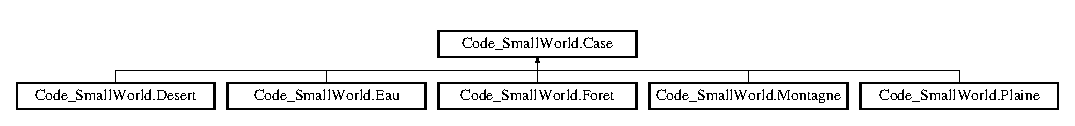
\includegraphics[height=1.244444cm]{interface_code___small_world_1_1_case}
\end{center}
\end{figure}


The documentation for this interface was generated from the following file\-:\begin{DoxyCompactItemize}
\item 
C\-:/\-Users/damienc/\-Documents/\-Git\-Hub/\-Small\-World/\-Visual\-Studio/\-Projet\-P\-O\-O/Case.\-cs\end{DoxyCompactItemize}

\hypertarget{class_code___small_world_1_1_class1}{\section{Code\-\_\-\-Small\-World.\-Class1 Class Reference}
\label{class_code___small_world_1_1_class1}\index{Code\-\_\-\-Small\-World.\-Class1@{Code\-\_\-\-Small\-World.\-Class1}}
}


The documentation for this class was generated from the following file\-:\begin{DoxyCompactItemize}
\item 
C\-:/\-Users/damienc/\-Documents/\-Git\-Hub/\-Small\-World/\-Visual\-Studio/\-Projet\-P\-O\-O/Class1.\-cs\end{DoxyCompactItemize}

\hypertarget{class_code___small_world_1_1_createur_partie}{\section{Code\-\_\-\-Small\-World.\-Createur\-Partie Class Reference}
\label{class_code___small_world_1_1_createur_partie}\index{Code\-\_\-\-Small\-World.\-Createur\-Partie@{Code\-\_\-\-Small\-World.\-Createur\-Partie}}
}
Inheritance diagram for Code\-\_\-\-Small\-World.\-Createur\-Partie\-:\begin{figure}[H]
\begin{center}
\leavevmode
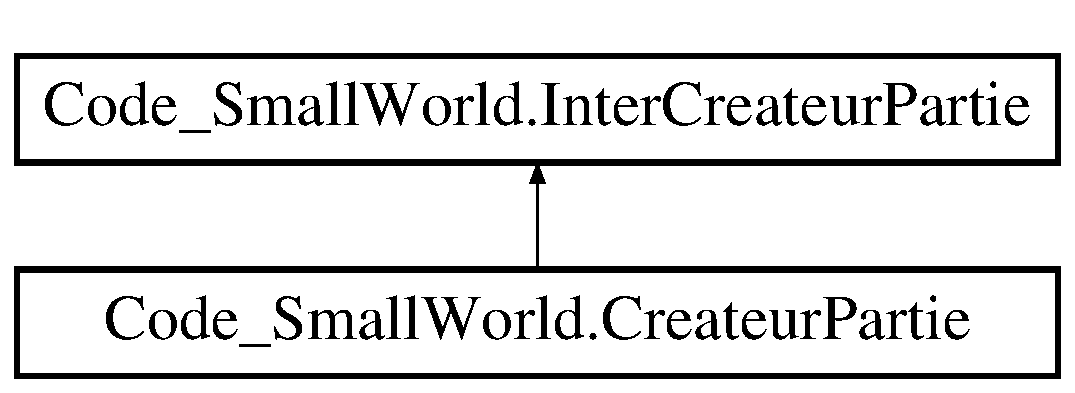
\includegraphics[height=2.000000cm]{class_code___small_world_1_1_createur_partie}
\end{center}
\end{figure}
\subsection*{Public Member Functions}
\begin{DoxyCompactItemize}
\item 
\hypertarget{class_code___small_world_1_1_createur_partie_a3836d8cd285e4cc0686d693dd91c18a5}{void {\bfseries construire} ()}\label{class_code___small_world_1_1_createur_partie_a3836d8cd285e4cc0686d693dd91c18a5}

\end{DoxyCompactItemize}
\subsection*{Properties}
\begin{DoxyCompactItemize}
\item 
\hypertarget{class_code___small_world_1_1_createur_partie_a3d566654338c6f3d15b65cc128424f88}{\hyperlink{class_code___small_world_1_1_monteur_partie}{Code\-\_\-\-Small\-World.\-Monteur\-Partie} {\bfseries Monteur\-Partie}\hspace{0.3cm}{\ttfamily  \mbox{[}get, set\mbox{]}}}\label{class_code___small_world_1_1_createur_partie_a3d566654338c6f3d15b65cc128424f88}

\end{DoxyCompactItemize}


The documentation for this class was generated from the following file\-:\begin{DoxyCompactItemize}
\item 
C\-:/\-Users/damienc/\-Documents/\-Git\-Hub/\-Small\-World/\-Visual\-Studio/\-Projet\-P\-O\-O/Createur\-Partie.\-cs\end{DoxyCompactItemize}

\hypertarget{interface_code___small_world_1_1_desert}{\section{Code\-\_\-\-Small\-World.\-Desert Interface Reference}
\label{interface_code___small_world_1_1_desert}\index{Code\-\_\-\-Small\-World.\-Desert@{Code\-\_\-\-Small\-World.\-Desert}}
}
Inheritance diagram for Code\-\_\-\-Small\-World.\-Desert\-:\begin{figure}[H]
\begin{center}
\leavevmode
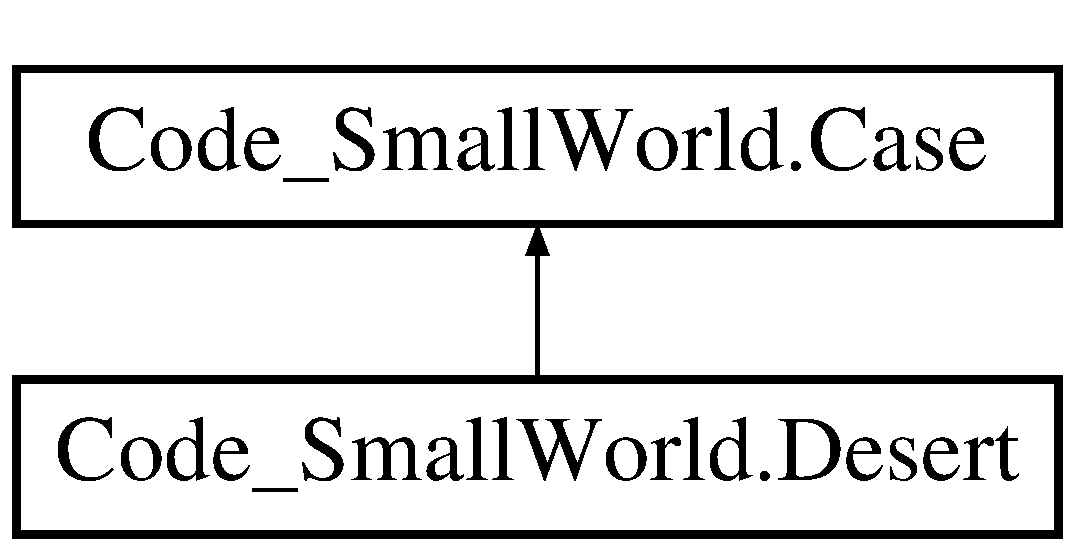
\includegraphics[height=2.000000cm]{interface_code___small_world_1_1_desert}
\end{center}
\end{figure}


The documentation for this interface was generated from the following file\-:\begin{DoxyCompactItemize}
\item 
C\-:/\-Users/damienc/\-Documents/\-Git\-Hub/\-Small\-World/\-Visual\-Studio/\-Projet\-P\-O\-O/desert.\-cs\end{DoxyCompactItemize}

\hypertarget{interface_code___small_world_1_1_eau}{\section{Code\-\_\-\-Small\-World.\-Eau Interface Reference}
\label{interface_code___small_world_1_1_eau}\index{Code\-\_\-\-Small\-World.\-Eau@{Code\-\_\-\-Small\-World.\-Eau}}
}
Inheritance diagram for Code\-\_\-\-Small\-World.\-Eau\-:\begin{figure}[H]
\begin{center}
\leavevmode
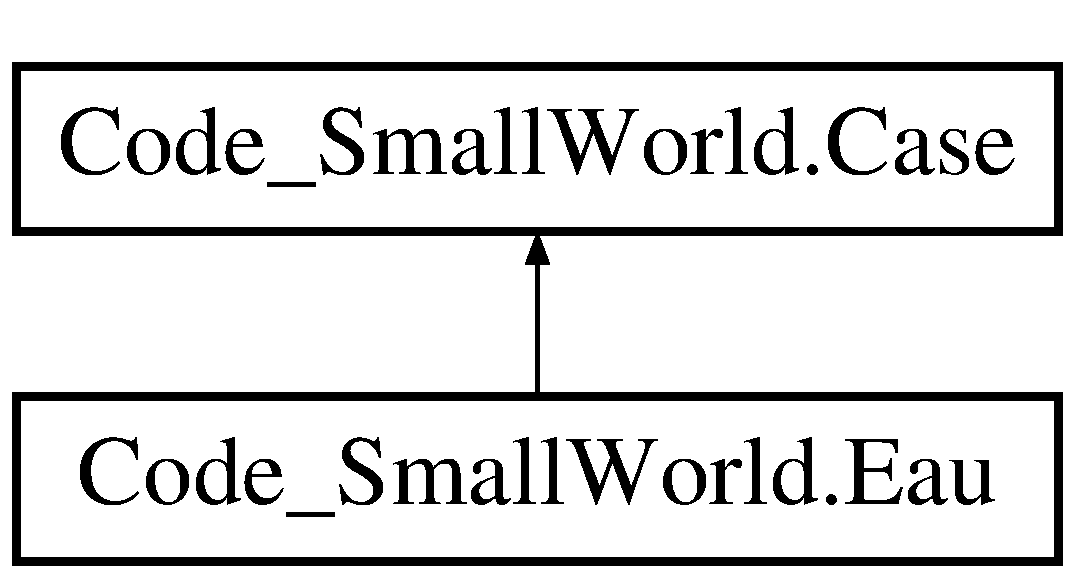
\includegraphics[height=2.000000cm]{interface_code___small_world_1_1_eau}
\end{center}
\end{figure}


The documentation for this interface was generated from the following file\-:\begin{DoxyCompactItemize}
\item 
C\-:/\-Users/damienc/\-Documents/\-Git\-Hub/\-Small\-World/\-Visual\-Studio/\-Projet\-P\-O\-O/eau.\-cs\end{DoxyCompactItemize}

\hypertarget{interface_code___small_world_1_1_fabrique___unite___gaulois}{\section{Code\-\_\-\-Small\-World.\-Fabrique\-\_\-\-Unite\-\_\-\-Gaulois Interface Reference}
\label{interface_code___small_world_1_1_fabrique___unite___gaulois}\index{Code\-\_\-\-Small\-World.\-Fabrique\-\_\-\-Unite\-\_\-\-Gaulois@{Code\-\_\-\-Small\-World.\-Fabrique\-\_\-\-Unite\-\_\-\-Gaulois}}
}
Inheritance diagram for Code\-\_\-\-Small\-World.\-Fabrique\-\_\-\-Unite\-\_\-\-Gaulois\-:\begin{figure}[H]
\begin{center}
\leavevmode
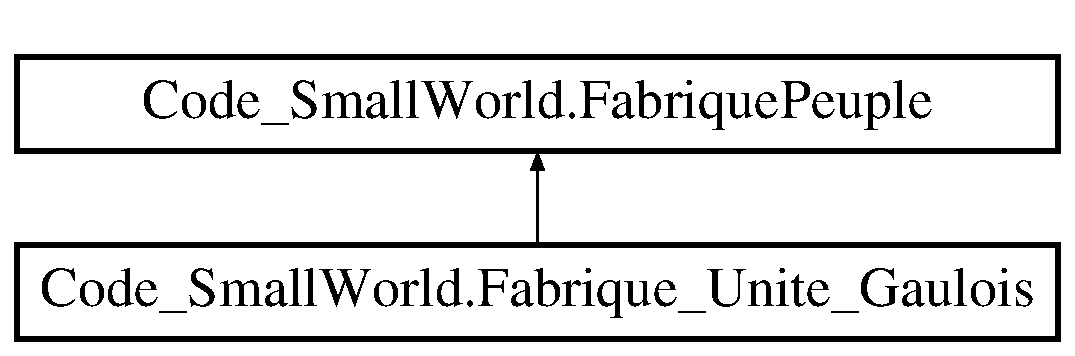
\includegraphics[height=2.000000cm]{interface_code___small_world_1_1_fabrique___unite___gaulois}
\end{center}
\end{figure}
\subsection*{Additional Inherited Members}


The documentation for this interface was generated from the following file\-:\begin{DoxyCompactItemize}
\item 
C\-:/\-Users/damienc/\-Documents/\-Git\-Hub/\-Small\-World/\-Visual\-Studio/\-Projet\-P\-O\-O/Fabrique\-Peuple.\-cs\end{DoxyCompactItemize}

\hypertarget{interface_code___small_world_1_1_fabrique___unite___nain}{\section{Code\-\_\-\-Small\-World.\-Fabrique\-\_\-\-Unite\-\_\-\-Nain Interface Reference}
\label{interface_code___small_world_1_1_fabrique___unite___nain}\index{Code\-\_\-\-Small\-World.\-Fabrique\-\_\-\-Unite\-\_\-\-Nain@{Code\-\_\-\-Small\-World.\-Fabrique\-\_\-\-Unite\-\_\-\-Nain}}
}
Inheritance diagram for Code\-\_\-\-Small\-World.\-Fabrique\-\_\-\-Unite\-\_\-\-Nain\-:\begin{figure}[H]
\begin{center}
\leavevmode
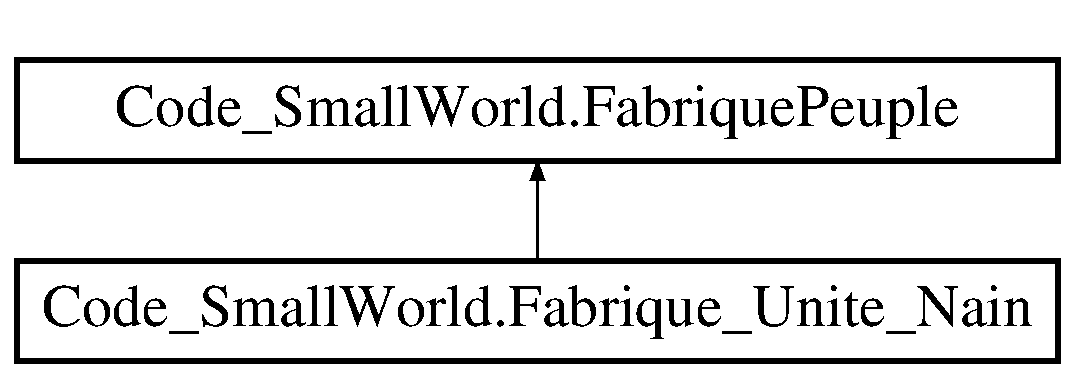
\includegraphics[height=2.000000cm]{interface_code___small_world_1_1_fabrique___unite___nain}
\end{center}
\end{figure}
\subsection*{Additional Inherited Members}


The documentation for this interface was generated from the following file\-:\begin{DoxyCompactItemize}
\item 
C\-:/\-Users/damienc/\-Documents/\-Git\-Hub/\-Small\-World/\-Visual\-Studio/\-Projet\-P\-O\-O/Fabrique\-Nain.\-cs\end{DoxyCompactItemize}

\hypertarget{interface_code___small_world_1_1_fabrique___unite___viking}{\section{Code\-\_\-\-Small\-World.\-Fabrique\-\_\-\-Unite\-\_\-\-Viking Interface Reference}
\label{interface_code___small_world_1_1_fabrique___unite___viking}\index{Code\-\_\-\-Small\-World.\-Fabrique\-\_\-\-Unite\-\_\-\-Viking@{Code\-\_\-\-Small\-World.\-Fabrique\-\_\-\-Unite\-\_\-\-Viking}}
}
Inheritance diagram for Code\-\_\-\-Small\-World.\-Fabrique\-\_\-\-Unite\-\_\-\-Viking\-:\begin{figure}[H]
\begin{center}
\leavevmode
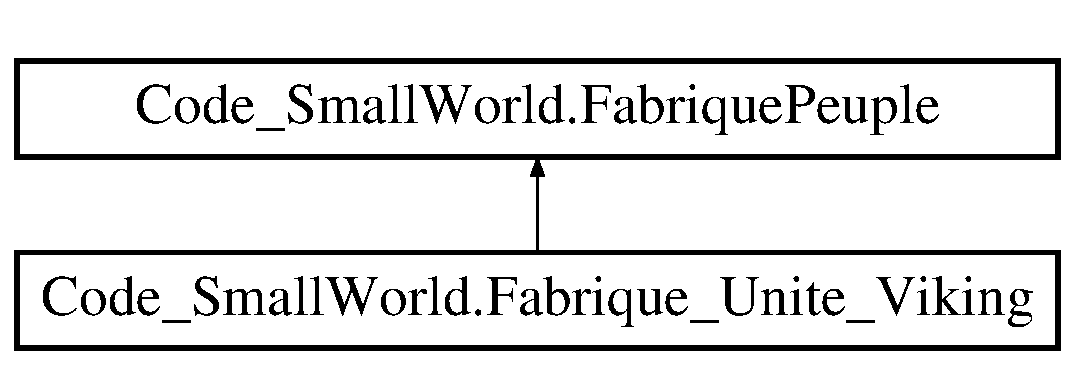
\includegraphics[height=2.000000cm]{interface_code___small_world_1_1_fabrique___unite___viking}
\end{center}
\end{figure}
\subsection*{Additional Inherited Members}


The documentation for this interface was generated from the following file\-:\begin{DoxyCompactItemize}
\item 
C\-:/\-Users/damienc/\-Documents/\-Git\-Hub/\-Small\-World/\-Visual\-Studio/\-Projet\-P\-O\-O/Fabrique\-Viking.\-cs\end{DoxyCompactItemize}

\hypertarget{interface_code___small_world_1_1_fabrique_case}{\section{Code\-\_\-\-Small\-World.\-Fabrique\-Case Interface Reference}
\label{interface_code___small_world_1_1_fabrique_case}\index{Code\-\_\-\-Small\-World.\-Fabrique\-Case@{Code\-\_\-\-Small\-World.\-Fabrique\-Case}}
}
\subsection*{Public Member Functions}
\begin{DoxyCompactItemize}
\item 
\hypertarget{interface_code___small_world_1_1_fabrique_case_ac65a293584f1cfd8651a58e187bdf5dd}{void {\bfseries obtenir\-Eau} ()}\label{interface_code___small_world_1_1_fabrique_case_ac65a293584f1cfd8651a58e187bdf5dd}

\item 
\hypertarget{interface_code___small_world_1_1_fabrique_case_abeece57e75e942ca601573afae892c72}{void {\bfseries obtenir\-Montagne} ()}\label{interface_code___small_world_1_1_fabrique_case_abeece57e75e942ca601573afae892c72}

\item 
\hypertarget{interface_code___small_world_1_1_fabrique_case_a0d940148059a5822c144060adc1cb35f}{void {\bfseries obtenir\-Desert} ()}\label{interface_code___small_world_1_1_fabrique_case_a0d940148059a5822c144060adc1cb35f}

\item 
\hypertarget{interface_code___small_world_1_1_fabrique_case_a834cb247f9b2cb44b5d7093f87fe02ca}{void {\bfseries obtenir\-Plaine} ()}\label{interface_code___small_world_1_1_fabrique_case_a834cb247f9b2cb44b5d7093f87fe02ca}

\item 
\hypertarget{interface_code___small_world_1_1_fabrique_case_a3f203d3e3c3e07f2b88de30858303db4}{void {\bfseries obtenir\-Foret} ()}\label{interface_code___small_world_1_1_fabrique_case_a3f203d3e3c3e07f2b88de30858303db4}

\item 
\hypertarget{interface_code___small_world_1_1_fabrique_case_a8ab2d827e269eabfd659d98a003f2a05}{void {\bfseries obtenir\-Case} ()}\label{interface_code___small_world_1_1_fabrique_case_a8ab2d827e269eabfd659d98a003f2a05}

\end{DoxyCompactItemize}


The documentation for this interface was generated from the following file\-:\begin{DoxyCompactItemize}
\item 
C\-:/\-Users/damienc/\-Documents/\-Git\-Hub/\-Small\-World/\-Visual\-Studio/\-Projet\-P\-O\-O/Fabrique\-Case.\-cs\end{DoxyCompactItemize}

\hypertarget{interface_code___small_world_1_1_fabrique_jeu}{\section{Code\-\_\-\-Small\-World.\-Fabrique\-Jeu Interface Reference}
\label{interface_code___small_world_1_1_fabrique_jeu}\index{Code\-\_\-\-Small\-World.\-Fabrique\-Jeu@{Code\-\_\-\-Small\-World.\-Fabrique\-Jeu}}
}
\subsection*{Public Member Functions}
\begin{DoxyCompactItemize}
\item 
\hypertarget{interface_code___small_world_1_1_fabrique_jeu_ae7b678cd987b4f77a19a272d65cf8fa4}{void {\bfseries creer\-Partie} ()}\label{interface_code___small_world_1_1_fabrique_jeu_ae7b678cd987b4f77a19a272d65cf8fa4}

\item 
\hypertarget{interface_code___small_world_1_1_fabrique_jeu_aad85073c518e20f457b8f7e50222c314}{void {\bfseries creer\-Joueur} (string nom\-Joueur, string \hyperlink{interface_code___small_world_1_1_peuple}{Peuple})}\label{interface_code___small_world_1_1_fabrique_jeu_aad85073c518e20f457b8f7e50222c314}

\item 
\hypertarget{interface_code___small_world_1_1_fabrique_jeu_aef37e4bf07611be63bb1b2c91c5dc5d1}{void {\bfseries charger\-Partie} ()}\label{interface_code___small_world_1_1_fabrique_jeu_aef37e4bf07611be63bb1b2c91c5dc5d1}

\end{DoxyCompactItemize}


The documentation for this interface was generated from the following file\-:\begin{DoxyCompactItemize}
\item 
C\-:/\-Users/damienc/\-Documents/\-Git\-Hub/\-Small\-World/\-Visual\-Studio/\-Projet\-P\-O\-O/Fabrique\-Jeu.\-cs\end{DoxyCompactItemize}

\hypertarget{interface_code___small_world_1_1_fabrique_peuple}{\section{Code\-\_\-\-Small\-World.\-Fabrique\-Peuple Interface Reference}
\label{interface_code___small_world_1_1_fabrique_peuple}\index{Code\-\_\-\-Small\-World.\-Fabrique\-Peuple@{Code\-\_\-\-Small\-World.\-Fabrique\-Peuple}}
}
Inheritance diagram for Code\-\_\-\-Small\-World.\-Fabrique\-Peuple\-:\begin{figure}[H]
\begin{center}
\leavevmode
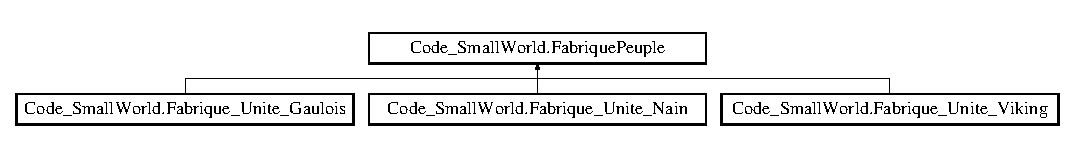
\includegraphics[height=1.447028cm]{interface_code___small_world_1_1_fabrique_peuple}
\end{center}
\end{figure}
\subsection*{Public Member Functions}
\begin{DoxyCompactItemize}
\item 
\hypertarget{interface_code___small_world_1_1_fabrique_peuple_a06a04cf83d40339635793d765e2917d1}{void {\bfseries fabriquer\-Peuple} ()}\label{interface_code___small_world_1_1_fabrique_peuple_a06a04cf83d40339635793d765e2917d1}

\end{DoxyCompactItemize}


The documentation for this interface was generated from the following file\-:\begin{DoxyCompactItemize}
\item 
C\-:/\-Users/damienc/\-Documents/\-Git\-Hub/\-Small\-World/\-Visual\-Studio/\-Projet\-P\-O\-O/Fabrique.\-cs\end{DoxyCompactItemize}

\hypertarget{interface_code___small_world_1_1_foret}{\section{Code\-\_\-\-Small\-World.\-Foret Interface Reference}
\label{interface_code___small_world_1_1_foret}\index{Code\-\_\-\-Small\-World.\-Foret@{Code\-\_\-\-Small\-World.\-Foret}}
}
Inheritance diagram for Code\-\_\-\-Small\-World.\-Foret\-:\begin{figure}[H]
\begin{center}
\leavevmode
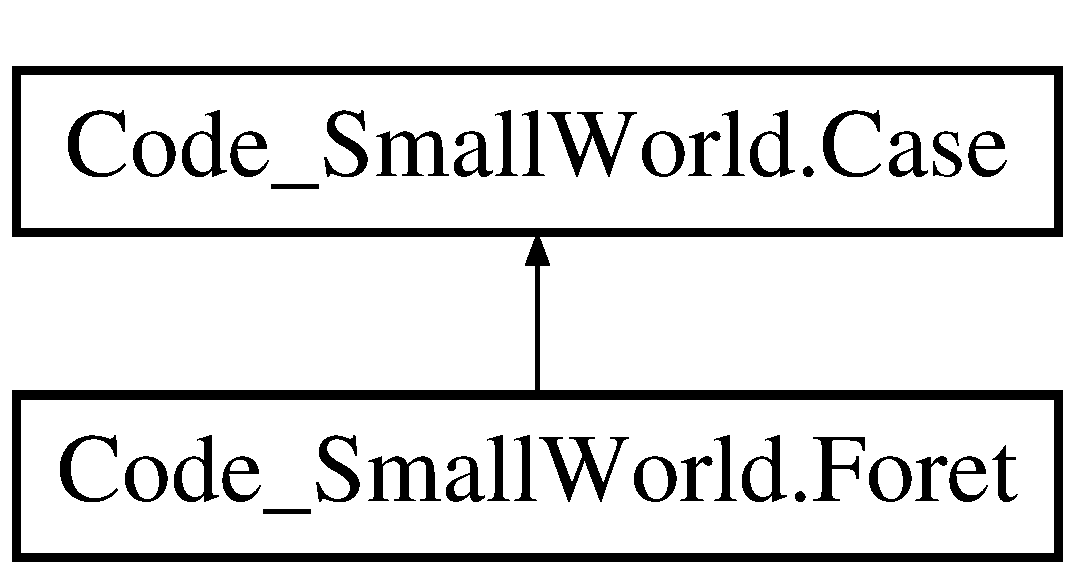
\includegraphics[height=2.000000cm]{interface_code___small_world_1_1_foret}
\end{center}
\end{figure}


The documentation for this interface was generated from the following file\-:\begin{DoxyCompactItemize}
\item 
C\-:/\-Users/damienc/\-Documents/\-Git\-Hub/\-Small\-World/\-Visual\-Studio/\-Projet\-P\-O\-O/foret.\-cs\end{DoxyCompactItemize}

\hypertarget{interface_code___small_world_1_1_inter_createur_partie}{\section{Code\-\_\-\-Small\-World.\-Inter\-Createur\-Partie Interface Reference}
\label{interface_code___small_world_1_1_inter_createur_partie}\index{Code\-\_\-\-Small\-World.\-Inter\-Createur\-Partie@{Code\-\_\-\-Small\-World.\-Inter\-Createur\-Partie}}
}
Inheritance diagram for Code\-\_\-\-Small\-World.\-Inter\-Createur\-Partie\-:\begin{figure}[H]
\begin{center}
\leavevmode
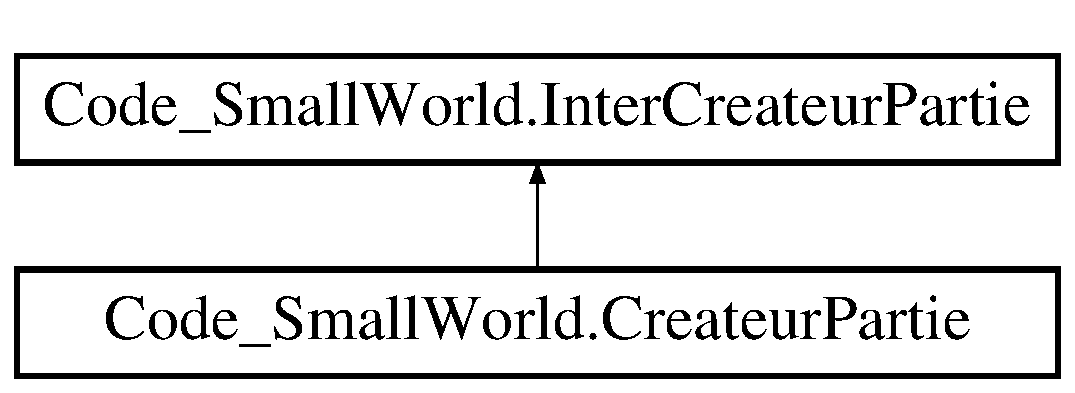
\includegraphics[height=2.000000cm]{interface_code___small_world_1_1_inter_createur_partie}
\end{center}
\end{figure}
\subsection*{Public Member Functions}
\begin{DoxyCompactItemize}
\item 
\hypertarget{interface_code___small_world_1_1_inter_createur_partie_a79e52693285229577bda38121484e779}{void {\bfseries construire} ()}\label{interface_code___small_world_1_1_inter_createur_partie_a79e52693285229577bda38121484e779}

\end{DoxyCompactItemize}


The documentation for this interface was generated from the following file\-:\begin{DoxyCompactItemize}
\item 
C\-:/\-Users/damienc/\-Documents/\-Git\-Hub/\-Small\-World/\-Visual\-Studio/\-Projet\-P\-O\-O/Createur\-Partie.\-cs\end{DoxyCompactItemize}

\hypertarget{interface_code___small_world_1_1_inter_monteur_partie}{\section{Code\-\_\-\-Small\-World.\-Inter\-Monteur\-Partie Interface Reference}
\label{interface_code___small_world_1_1_inter_monteur_partie}\index{Code\-\_\-\-Small\-World.\-Inter\-Monteur\-Partie@{Code\-\_\-\-Small\-World.\-Inter\-Monteur\-Partie}}
}
Inheritance diagram for Code\-\_\-\-Small\-World.\-Inter\-Monteur\-Partie\-:\begin{figure}[H]
\begin{center}
\leavevmode
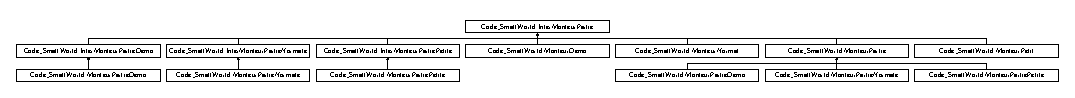
\includegraphics[height=0.869565cm]{interface_code___small_world_1_1_inter_monteur_partie}
\end{center}
\end{figure}
\subsection*{Public Member Functions}
\begin{DoxyCompactItemize}
\item 
\hypertarget{interface_code___small_world_1_1_inter_monteur_partie_a8f07e29ce6ab00e90ebc49ab92f795ce}{\hyperlink{interface_code___small_world_1_1_partie}{Partie} {\bfseries creer\-Partie} ()}\label{interface_code___small_world_1_1_inter_monteur_partie_a8f07e29ce6ab00e90ebc49ab92f795ce}

\item 
\hypertarget{interface_code___small_world_1_1_inter_monteur_partie_adae897749a4c19c7d6b545f8157c9235}{void {\bfseries ajouter\-Carte} ()}\label{interface_code___small_world_1_1_inter_monteur_partie_adae897749a4c19c7d6b545f8157c9235}

\item 
\hypertarget{interface_code___small_world_1_1_inter_monteur_partie_a6443110e45d388d55b2cb8e23db2aa1c}{void {\bfseries ajouter\-Joueur} ()}\label{interface_code___small_world_1_1_inter_monteur_partie_a6443110e45d388d55b2cb8e23db2aa1c}

\item 
\hypertarget{interface_code___small_world_1_1_inter_monteur_partie_ae8f34805f85b6c55380b944f67752498}{void {\bfseries placer\-Unites} ()}\label{interface_code___small_world_1_1_inter_monteur_partie_ae8f34805f85b6c55380b944f67752498}

\end{DoxyCompactItemize}


The documentation for this interface was generated from the following file\-:\begin{DoxyCompactItemize}
\item 
C\-:/\-Users/damienc/\-Documents/\-Git\-Hub/\-Small\-World/\-Visual\-Studio/\-Projet\-P\-O\-O/Monteur\-Carte.\-cs\end{DoxyCompactItemize}

\hypertarget{interface_code___small_world_1_1_inter_monteur_partie_demo}{\section{Code\-\_\-\-Small\-World.\-Inter\-Monteur\-Partie\-Demo Interface Reference}
\label{interface_code___small_world_1_1_inter_monteur_partie_demo}\index{Code\-\_\-\-Small\-World.\-Inter\-Monteur\-Partie\-Demo@{Code\-\_\-\-Small\-World.\-Inter\-Monteur\-Partie\-Demo}}
}
Inheritance diagram for Code\-\_\-\-Small\-World.\-Inter\-Monteur\-Partie\-Demo\-:\begin{figure}[H]
\begin{center}
\leavevmode
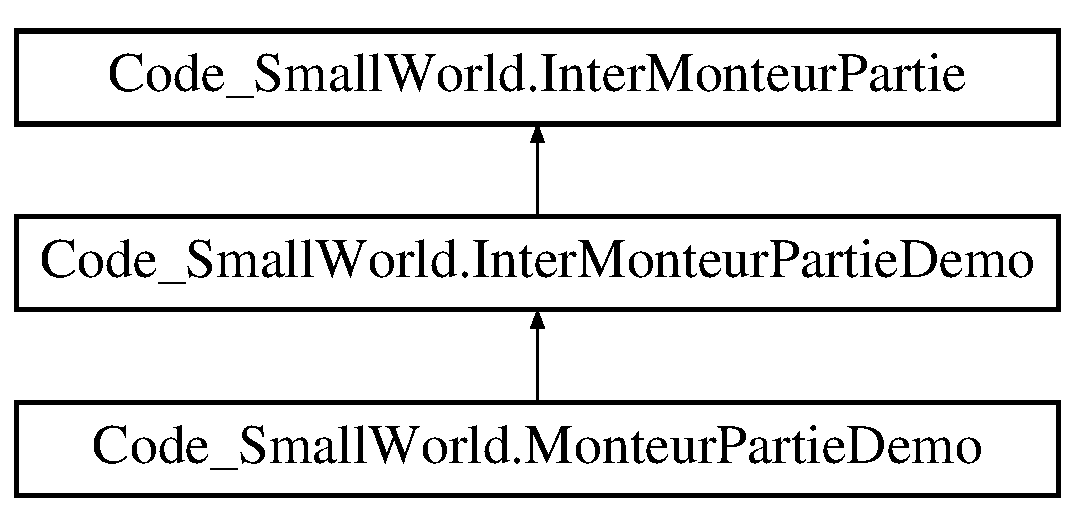
\includegraphics[height=3.000000cm]{interface_code___small_world_1_1_inter_monteur_partie_demo}
\end{center}
\end{figure}
\subsection*{Public Member Functions}
\begin{DoxyCompactItemize}
\item 
\hypertarget{interface_code___small_world_1_1_inter_monteur_partie_demo_aae0ae232e14a6051532071bb40d42aad}{void {\bfseries ajouter\-Peuple} ()}\label{interface_code___small_world_1_1_inter_monteur_partie_demo_aae0ae232e14a6051532071bb40d42aad}

\end{DoxyCompactItemize}


The documentation for this interface was generated from the following file\-:\begin{DoxyCompactItemize}
\item 
C\-:/\-Users/damienc/\-Documents/\-Git\-Hub/\-Small\-World/\-Visual\-Studio/\-Projet\-P\-O\-O/Monteur\-Partie\-Demo.\-cs\end{DoxyCompactItemize}

\hypertarget{interface_code___small_world_1_1_inter_monteur_partie_normale}{\section{Code\-\_\-\-Small\-World.\-Inter\-Monteur\-Partie\-Normale Interface Reference}
\label{interface_code___small_world_1_1_inter_monteur_partie_normale}\index{Code\-\_\-\-Small\-World.\-Inter\-Monteur\-Partie\-Normale@{Code\-\_\-\-Small\-World.\-Inter\-Monteur\-Partie\-Normale}}
}
Inheritance diagram for Code\-\_\-\-Small\-World.\-Inter\-Monteur\-Partie\-Normale\-:\begin{figure}[H]
\begin{center}
\leavevmode
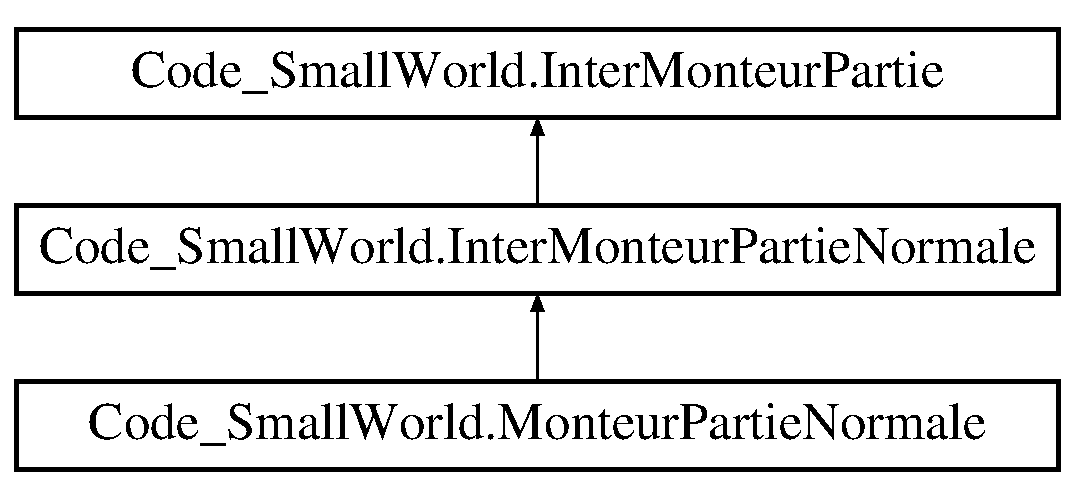
\includegraphics[height=3.000000cm]{interface_code___small_world_1_1_inter_monteur_partie_normale}
\end{center}
\end{figure}
\subsection*{Public Member Functions}
\begin{DoxyCompactItemize}
\item 
\hypertarget{interface_code___small_world_1_1_inter_monteur_partie_normale_a813c0455bcaf98b5e35260846d80f825}{void {\bfseries ajouter\-Peuple} ()}\label{interface_code___small_world_1_1_inter_monteur_partie_normale_a813c0455bcaf98b5e35260846d80f825}

\end{DoxyCompactItemize}


The documentation for this interface was generated from the following file\-:\begin{DoxyCompactItemize}
\item 
C\-:/\-Users/damienc/\-Documents/\-Git\-Hub/\-Small\-World/\-Visual\-Studio/\-Projet\-P\-O\-O/Monteur\-Partie\-Normale.\-cs\end{DoxyCompactItemize}

\hypertarget{interface_code___small_world_1_1_inter_monteur_partie_petite}{\section{Code\-\_\-\-Small\-World.\-Inter\-Monteur\-Partie\-Petite Interface Reference}
\label{interface_code___small_world_1_1_inter_monteur_partie_petite}\index{Code\-\_\-\-Small\-World.\-Inter\-Monteur\-Partie\-Petite@{Code\-\_\-\-Small\-World.\-Inter\-Monteur\-Partie\-Petite}}
}
Inheritance diagram for Code\-\_\-\-Small\-World.\-Inter\-Monteur\-Partie\-Petite\-:\begin{figure}[H]
\begin{center}
\leavevmode
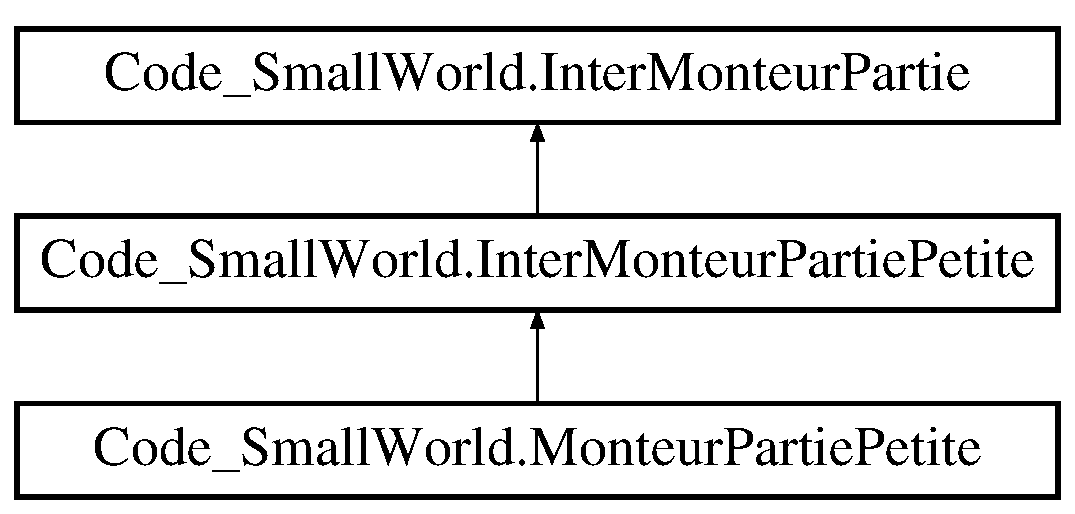
\includegraphics[height=3.000000cm]{interface_code___small_world_1_1_inter_monteur_partie_petite}
\end{center}
\end{figure}
\subsection*{Public Member Functions}
\begin{DoxyCompactItemize}
\item 
\hypertarget{interface_code___small_world_1_1_inter_monteur_partie_petite_a136baa469738fc9c5b855e217236ce9a}{void {\bfseries ajouter\-Peuple} ()}\label{interface_code___small_world_1_1_inter_monteur_partie_petite_a136baa469738fc9c5b855e217236ce9a}

\end{DoxyCompactItemize}


The documentation for this interface was generated from the following file\-:\begin{DoxyCompactItemize}
\item 
C\-:/\-Users/damienc/\-Documents/\-Git\-Hub/\-Small\-World/\-Visual\-Studio/\-Projet\-P\-O\-O/Monteur\-Partie\-Petite.\-cs\end{DoxyCompactItemize}

\hypertarget{interface_code___small_world_1_1_joueur}{\section{Code\-\_\-\-Small\-World.\-Joueur Interface Reference}
\label{interface_code___small_world_1_1_joueur}\index{Code\-\_\-\-Small\-World.\-Joueur@{Code\-\_\-\-Small\-World.\-Joueur}}
}


The documentation for this interface was generated from the following file\-:\begin{DoxyCompactItemize}
\item 
C\-:/\-Users/damienc/\-Documents/\-Git\-Hub/\-Small\-World/\-Visual\-Studio/\-Projet\-P\-O\-O/Joueur.\-cs\end{DoxyCompactItemize}

\hypertarget{interface_code___small_world_1_1_montagne}{\section{Code\-\_\-\-Small\-World.\-Montagne Interface Reference}
\label{interface_code___small_world_1_1_montagne}\index{Code\-\_\-\-Small\-World.\-Montagne@{Code\-\_\-\-Small\-World.\-Montagne}}
}
Inheritance diagram for Code\-\_\-\-Small\-World.\-Montagne\-:\begin{figure}[H]
\begin{center}
\leavevmode
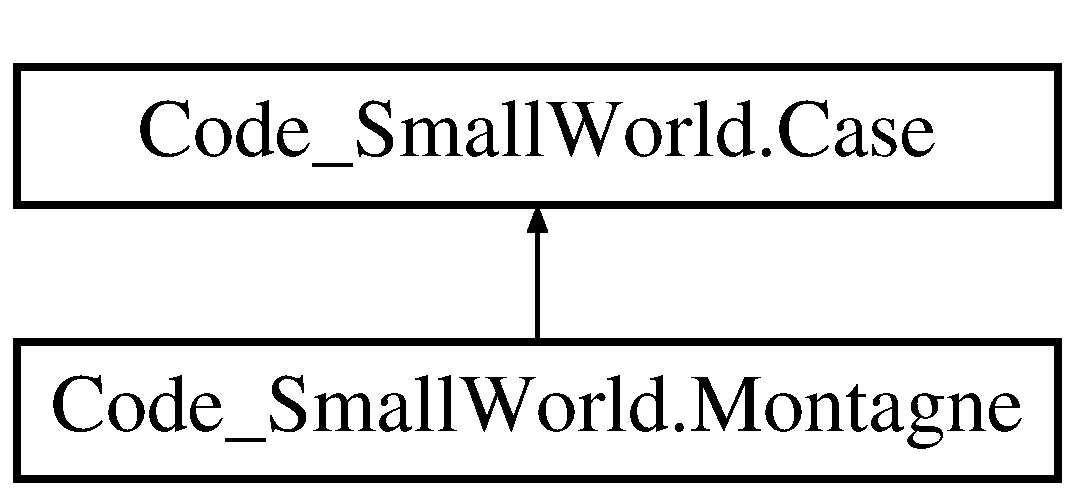
\includegraphics[height=2.000000cm]{interface_code___small_world_1_1_montagne}
\end{center}
\end{figure}


The documentation for this interface was generated from the following file\-:\begin{DoxyCompactItemize}
\item 
C\-:/\-Users/damienc/\-Documents/\-Git\-Hub/\-Small\-World/\-Visual\-Studio/\-Projet\-P\-O\-O/montagne.\-cs\end{DoxyCompactItemize}

\hypertarget{interface_code___small_world_1_1_monteur_demo}{\section{Code\-\_\-\-Small\-World.\-Monteur\-Demo Interface Reference}
\label{interface_code___small_world_1_1_monteur_demo}\index{Code\-\_\-\-Small\-World.\-Monteur\-Demo@{Code\-\_\-\-Small\-World.\-Monteur\-Demo}}
}
Inheritance diagram for Code\-\_\-\-Small\-World.\-Monteur\-Demo\-:\begin{figure}[H]
\begin{center}
\leavevmode
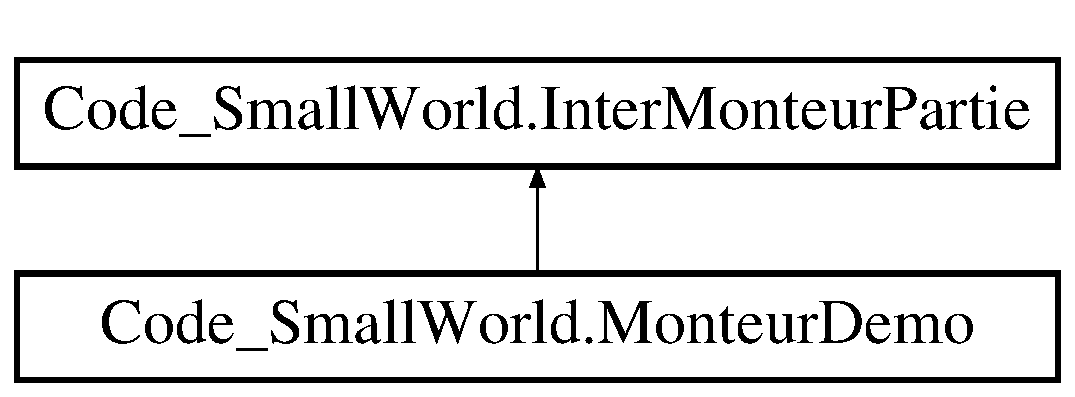
\includegraphics[height=2.000000cm]{interface_code___small_world_1_1_monteur_demo}
\end{center}
\end{figure}
\subsection*{Additional Inherited Members}


The documentation for this interface was generated from the following file\-:\begin{DoxyCompactItemize}
\item 
C\-:/\-Users/damienc/\-Documents/\-Git\-Hub/\-Small\-World/\-Visual\-Studio/\-Projet\-P\-O\-O/Monteur\-Demo.\-cs\end{DoxyCompactItemize}

\hypertarget{interface_code___small_world_1_1_monteur_normal}{\section{Code\-\_\-\-Small\-World.\-Monteur\-Normal Interface Reference}
\label{interface_code___small_world_1_1_monteur_normal}\index{Code\-\_\-\-Small\-World.\-Monteur\-Normal@{Code\-\_\-\-Small\-World.\-Monteur\-Normal}}
}
Inheritance diagram for Code\-\_\-\-Small\-World.\-Monteur\-Normal\-:\begin{figure}[H]
\begin{center}
\leavevmode
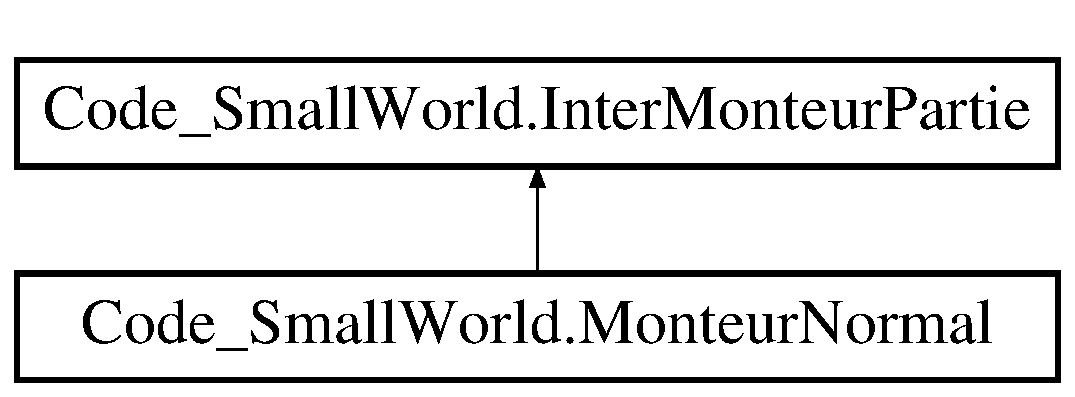
\includegraphics[height=2.000000cm]{interface_code___small_world_1_1_monteur_normal}
\end{center}
\end{figure}
\subsection*{Additional Inherited Members}


The documentation for this interface was generated from the following file\-:\begin{DoxyCompactItemize}
\item 
C\-:/\-Users/damienc/\-Documents/\-Git\-Hub/\-Small\-World/\-Visual\-Studio/\-Projet\-P\-O\-O/Monteur\-Normal.\-cs\end{DoxyCompactItemize}

\hypertarget{class_code___small_world_1_1_monteur_partie}{\section{Code\-\_\-\-Small\-World.\-Monteur\-Partie Class Reference}
\label{class_code___small_world_1_1_monteur_partie}\index{Code\-\_\-\-Small\-World.\-Monteur\-Partie@{Code\-\_\-\-Small\-World.\-Monteur\-Partie}}
}
Inheritance diagram for Code\-\_\-\-Small\-World.\-Monteur\-Partie\-:\begin{figure}[H]
\begin{center}
\leavevmode
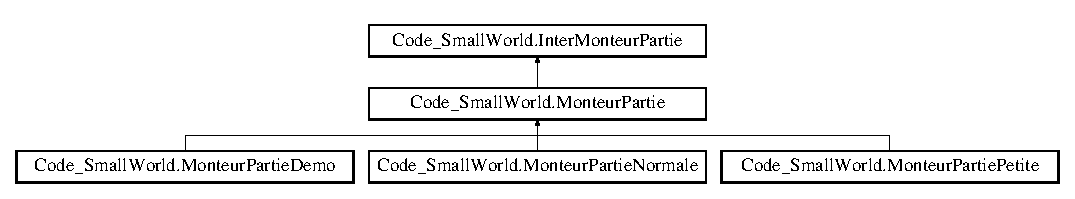
\includegraphics[height=2.231076cm]{class_code___small_world_1_1_monteur_partie}
\end{center}
\end{figure}
\subsection*{Public Member Functions}
\begin{DoxyCompactItemize}
\item 
\hypertarget{class_code___small_world_1_1_monteur_partie_a3ed8eb95a46eb27321ebc89a61c92920}{\hyperlink{interface_code___small_world_1_1_partie}{Code\-\_\-\-Small\-World.\-Partie} {\bfseries creer\-Partie} ()}\label{class_code___small_world_1_1_monteur_partie_a3ed8eb95a46eb27321ebc89a61c92920}

\item 
\hypertarget{class_code___small_world_1_1_monteur_partie_a2fd91bc4e3753c27c41d03e0d46a7882}{void {\bfseries ajouter\-Carte} ()}\label{class_code___small_world_1_1_monteur_partie_a2fd91bc4e3753c27c41d03e0d46a7882}

\item 
\hypertarget{class_code___small_world_1_1_monteur_partie_a4370c4d48c0e2d97611d3d449710fb1b}{void {\bfseries ajouter\-Joueur} ()}\label{class_code___small_world_1_1_monteur_partie_a4370c4d48c0e2d97611d3d449710fb1b}

\item 
\hypertarget{class_code___small_world_1_1_monteur_partie_a3bedbbf4bae673e8d817cc4fab26dde3}{void {\bfseries placer\-Unites} ()}\label{class_code___small_world_1_1_monteur_partie_a3bedbbf4bae673e8d817cc4fab26dde3}

\end{DoxyCompactItemize}


The documentation for this class was generated from the following file\-:\begin{DoxyCompactItemize}
\item 
C\-:/\-Users/damienc/\-Documents/\-Git\-Hub/\-Small\-World/\-Visual\-Studio/\-Projet\-P\-O\-O/Monteur\-Partie.\-cs\end{DoxyCompactItemize}

\hypertarget{class_code___small_world_1_1_monteur_partie_demo}{\section{Code\-\_\-\-Small\-World.\-Monteur\-Partie\-Demo Class Reference}
\label{class_code___small_world_1_1_monteur_partie_demo}\index{Code\-\_\-\-Small\-World.\-Monteur\-Partie\-Demo@{Code\-\_\-\-Small\-World.\-Monteur\-Partie\-Demo}}
}
Inheritance diagram for Code\-\_\-\-Small\-World.\-Monteur\-Partie\-Demo\-:\begin{figure}[H]
\begin{center}
\leavevmode
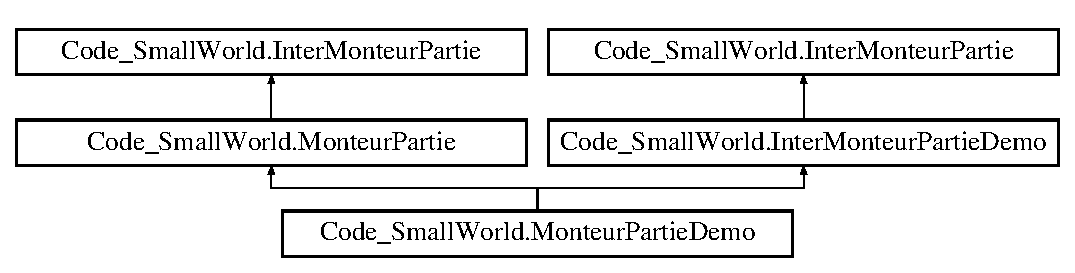
\includegraphics[height=3.000000cm]{class_code___small_world_1_1_monteur_partie_demo}
\end{center}
\end{figure}
\subsection*{Public Member Functions}
\begin{DoxyCompactItemize}
\item 
\hypertarget{class_code___small_world_1_1_monteur_partie_demo_a9a44ef267e3b9fa5b0fef9c680d916bd}{void {\bfseries ajouter\-Peuple} ()}\label{class_code___small_world_1_1_monteur_partie_demo_a9a44ef267e3b9fa5b0fef9c680d916bd}

\item 
\hypertarget{class_code___small_world_1_1_monteur_partie_demo_ac579027091c0f053adba26e9a597b4f5}{\hyperlink{interface_code___small_world_1_1_partie}{Code\-\_\-\-Small\-World.\-Partie} {\bfseries creer\-Partie} ()}\label{class_code___small_world_1_1_monteur_partie_demo_ac579027091c0f053adba26e9a597b4f5}

\item 
\hypertarget{class_code___small_world_1_1_monteur_partie_demo_afb127c1d1899948b1eaa4d08531cff94}{void {\bfseries ajouter\-Carte} ()}\label{class_code___small_world_1_1_monteur_partie_demo_afb127c1d1899948b1eaa4d08531cff94}

\item 
\hypertarget{class_code___small_world_1_1_monteur_partie_demo_a2dd24075e89d51b67b350b364e06f764}{void {\bfseries ajouter\-Joueur} ()}\label{class_code___small_world_1_1_monteur_partie_demo_a2dd24075e89d51b67b350b364e06f764}

\item 
\hypertarget{class_code___small_world_1_1_monteur_partie_demo_ac4e3b1234bf35dc370344a0f92cd1fed}{void {\bfseries placer\-Unites} ()}\label{class_code___small_world_1_1_monteur_partie_demo_ac4e3b1234bf35dc370344a0f92cd1fed}

\end{DoxyCompactItemize}


The documentation for this class was generated from the following file\-:\begin{DoxyCompactItemize}
\item 
C\-:/\-Users/damienc/\-Documents/\-Git\-Hub/\-Small\-World/\-Visual\-Studio/\-Projet\-P\-O\-O/Monteur\-Partie\-Demo.\-cs\end{DoxyCompactItemize}

\hypertarget{class_code___small_world_1_1_monteur_partie_normale}{\section{Code\-\_\-\-Small\-World.\-Monteur\-Partie\-Normale Class Reference}
\label{class_code___small_world_1_1_monteur_partie_normale}\index{Code\-\_\-\-Small\-World.\-Monteur\-Partie\-Normale@{Code\-\_\-\-Small\-World.\-Monteur\-Partie\-Normale}}
}
Inheritance diagram for Code\-\_\-\-Small\-World.\-Monteur\-Partie\-Normale\-:\begin{figure}[H]
\begin{center}
\leavevmode
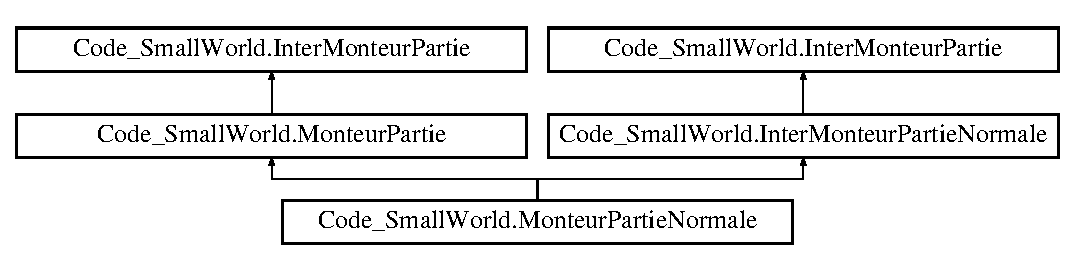
\includegraphics[height=3.000000cm]{class_code___small_world_1_1_monteur_partie_normale}
\end{center}
\end{figure}
\subsection*{Public Member Functions}
\begin{DoxyCompactItemize}
\item 
\hypertarget{class_code___small_world_1_1_monteur_partie_normale_af5450316c27e580d2de37f21d140863b}{void {\bfseries ajouter\-Peuple} ()}\label{class_code___small_world_1_1_monteur_partie_normale_af5450316c27e580d2de37f21d140863b}

\item 
\hypertarget{class_code___small_world_1_1_monteur_partie_normale_ad962266a5b272be6c4d01e91c8ded1cc}{\hyperlink{interface_code___small_world_1_1_partie}{Code\-\_\-\-Small\-World.\-Partie} {\bfseries creer\-Partie} ()}\label{class_code___small_world_1_1_monteur_partie_normale_ad962266a5b272be6c4d01e91c8ded1cc}

\item 
\hypertarget{class_code___small_world_1_1_monteur_partie_normale_ad17c12a99177de2562802a6f0f8f1a08}{void {\bfseries ajouter\-Carte} ()}\label{class_code___small_world_1_1_monteur_partie_normale_ad17c12a99177de2562802a6f0f8f1a08}

\item 
\hypertarget{class_code___small_world_1_1_monteur_partie_normale_a9487b01a5f55d9a33b34d77df503bbf1}{void {\bfseries ajouter\-Joueur} ()}\label{class_code___small_world_1_1_monteur_partie_normale_a9487b01a5f55d9a33b34d77df503bbf1}

\item 
\hypertarget{class_code___small_world_1_1_monteur_partie_normale_a00af0190687d4dcf96cf3c208ede5192}{void {\bfseries placer\-Unites} ()}\label{class_code___small_world_1_1_monteur_partie_normale_a00af0190687d4dcf96cf3c208ede5192}

\end{DoxyCompactItemize}


The documentation for this class was generated from the following file\-:\begin{DoxyCompactItemize}
\item 
C\-:/\-Users/damienc/\-Documents/\-Git\-Hub/\-Small\-World/\-Visual\-Studio/\-Projet\-P\-O\-O/Monteur\-Partie\-Normale.\-cs\end{DoxyCompactItemize}

\hypertarget{class_code___small_world_1_1_monteur_partie_petite}{\section{Code\-\_\-\-Small\-World.\-Monteur\-Partie\-Petite Class Reference}
\label{class_code___small_world_1_1_monteur_partie_petite}\index{Code\-\_\-\-Small\-World.\-Monteur\-Partie\-Petite@{Code\-\_\-\-Small\-World.\-Monteur\-Partie\-Petite}}
}
Inheritance diagram for Code\-\_\-\-Small\-World.\-Monteur\-Partie\-Petite\-:\begin{figure}[H]
\begin{center}
\leavevmode
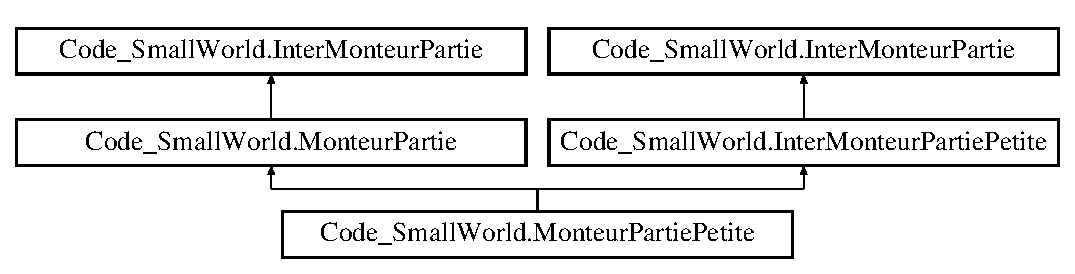
\includegraphics[height=3.000000cm]{class_code___small_world_1_1_monteur_partie_petite}
\end{center}
\end{figure}
\subsection*{Public Member Functions}
\begin{DoxyCompactItemize}
\item 
\hypertarget{class_code___small_world_1_1_monteur_partie_petite_a57934695a8b31d8b0e6a41c857f7da0f}{void {\bfseries ajouter\-Peuple} ()}\label{class_code___small_world_1_1_monteur_partie_petite_a57934695a8b31d8b0e6a41c857f7da0f}

\item 
\hypertarget{class_code___small_world_1_1_monteur_partie_petite_abd1097b50ddf84aaaa4eaaea598602e1}{\hyperlink{interface_code___small_world_1_1_partie}{Code\-\_\-\-Small\-World.\-Partie} {\bfseries creer\-Partie} ()}\label{class_code___small_world_1_1_monteur_partie_petite_abd1097b50ddf84aaaa4eaaea598602e1}

\item 
\hypertarget{class_code___small_world_1_1_monteur_partie_petite_ab14531d369212c8c67d2e7e52bd5a362}{void {\bfseries ajouter\-Carte} ()}\label{class_code___small_world_1_1_monteur_partie_petite_ab14531d369212c8c67d2e7e52bd5a362}

\item 
\hypertarget{class_code___small_world_1_1_monteur_partie_petite_aafe9f2e29347986daea49e95d4778096}{void {\bfseries ajouter\-Joueur} ()}\label{class_code___small_world_1_1_monteur_partie_petite_aafe9f2e29347986daea49e95d4778096}

\item 
\hypertarget{class_code___small_world_1_1_monteur_partie_petite_a0a57d5e7eeed60d8f4621851fc075fb2}{void {\bfseries placer\-Unites} ()}\label{class_code___small_world_1_1_monteur_partie_petite_a0a57d5e7eeed60d8f4621851fc075fb2}

\end{DoxyCompactItemize}


The documentation for this class was generated from the following file\-:\begin{DoxyCompactItemize}
\item 
C\-:/\-Users/damienc/\-Documents/\-Git\-Hub/\-Small\-World/\-Visual\-Studio/\-Projet\-P\-O\-O/Monteur\-Partie\-Petite.\-cs\end{DoxyCompactItemize}

\hypertarget{interface_code___small_world_1_1_monteur_petit}{\section{Code\-\_\-\-Small\-World.\-Monteur\-Petit Interface Reference}
\label{interface_code___small_world_1_1_monteur_petit}\index{Code\-\_\-\-Small\-World.\-Monteur\-Petit@{Code\-\_\-\-Small\-World.\-Monteur\-Petit}}
}
Inheritance diagram for Code\-\_\-\-Small\-World.\-Monteur\-Petit\-:\begin{figure}[H]
\begin{center}
\leavevmode
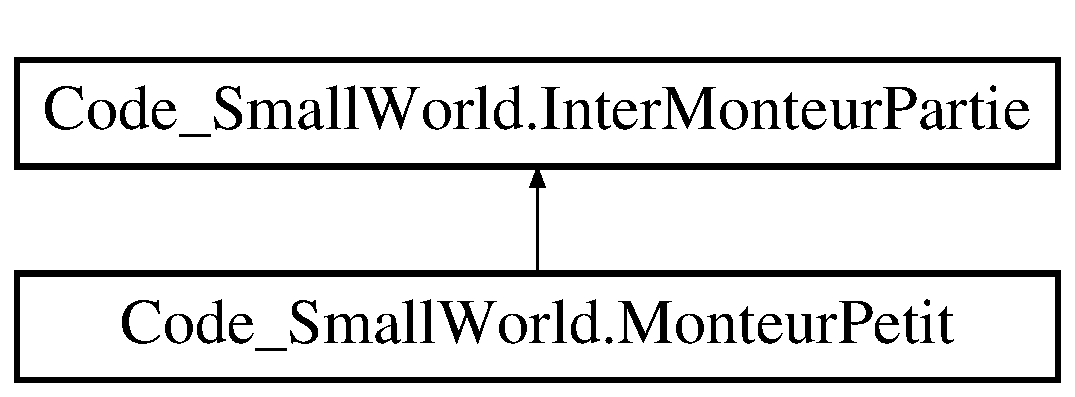
\includegraphics[height=2.000000cm]{interface_code___small_world_1_1_monteur_petit}
\end{center}
\end{figure}
\subsection*{Additional Inherited Members}


The documentation for this interface was generated from the following file\-:\begin{DoxyCompactItemize}
\item 
C\-:/\-Users/damienc/\-Documents/\-Git\-Hub/\-Small\-World/\-Visual\-Studio/\-Projet\-P\-O\-O/Monteur\-Petit.\-cs\end{DoxyCompactItemize}

\hypertarget{interface_code___small_world_1_1_nain}{\section{Code\-\_\-\-Small\-World.\-Nain Interface Reference}
\label{interface_code___small_world_1_1_nain}\index{Code\-\_\-\-Small\-World.\-Nain@{Code\-\_\-\-Small\-World.\-Nain}}
}


The documentation for this interface was generated from the following file\-:\begin{DoxyCompactItemize}
\item 
C\-:/\-Users/damienc/\-Documents/\-Git\-Hub/\-Small\-World/\-Visual\-Studio/\-Projet\-P\-O\-O/Nain.\-cs\end{DoxyCompactItemize}

\hypertarget{interface_code___small_world_1_1_partie}{\section{Code\-\_\-\-Small\-World.\-Partie Interface Reference}
\label{interface_code___small_world_1_1_partie}\index{Code\-\_\-\-Small\-World.\-Partie@{Code\-\_\-\-Small\-World.\-Partie}}
}


The documentation for this interface was generated from the following file\-:\begin{DoxyCompactItemize}
\item 
C\-:/\-Users/damienc/\-Documents/\-Git\-Hub/\-Small\-World/\-Visual\-Studio/\-Projet\-P\-O\-O/Partie.\-cs\end{DoxyCompactItemize}

\hypertarget{interface_code___small_world_1_1_peuple}{\section{Code\-\_\-\-Small\-World.\-Peuple Interface Reference}
\label{interface_code___small_world_1_1_peuple}\index{Code\-\_\-\-Small\-World.\-Peuple@{Code\-\_\-\-Small\-World.\-Peuple}}
}
Inheritance diagram for Code\-\_\-\-Small\-World.\-Peuple\-:\begin{figure}[H]
\begin{center}
\leavevmode
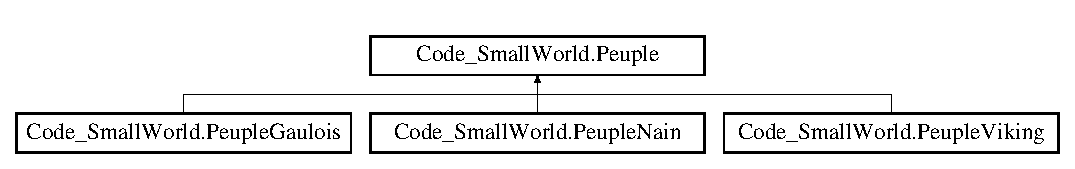
\includegraphics[height=1.821138cm]{interface_code___small_world_1_1_peuple}
\end{center}
\end{figure}
\subsection*{Public Member Functions}
\begin{DoxyCompactItemize}
\item 
\hypertarget{interface_code___small_world_1_1_peuple_adf261cd5244f9de0308f8257dedccbda}{\hyperlink{interface_code___small_world_1_1_unite}{Unite} {\bfseries creer\-Unite} ()}\label{interface_code___small_world_1_1_peuple_adf261cd5244f9de0308f8257dedccbda}

\end{DoxyCompactItemize}


The documentation for this interface was generated from the following file\-:\begin{DoxyCompactItemize}
\item 
C\-:/\-Users/damienc/\-Documents/\-Git\-Hub/\-Small\-World/\-Visual\-Studio/\-Projet\-P\-O\-O/Peuple.\-cs\end{DoxyCompactItemize}

\hypertarget{interface_code___small_world_1_1_peuple_g}{\section{Code\-\_\-\-Small\-World.\-Peuple\-G Interface Reference}
\label{interface_code___small_world_1_1_peuple_g}\index{Code\-\_\-\-Small\-World.\-Peuple\-G@{Code\-\_\-\-Small\-World.\-Peuple\-G}}
}


The documentation for this interface was generated from the following file\-:\begin{DoxyCompactItemize}
\item 
C\-:/\-Users/damienc/\-Documents/\-Git\-Hub/\-Small\-World/\-Visual\-Studio/\-Projet\-P\-O\-O/Peuple\-G.\-cs\end{DoxyCompactItemize}

\hypertarget{interface_code___small_world_1_1_peuple_gaulois}{\section{Code\-\_\-\-Small\-World.\-Peuple\-Gaulois Interface Reference}
\label{interface_code___small_world_1_1_peuple_gaulois}\index{Code\-\_\-\-Small\-World.\-Peuple\-Gaulois@{Code\-\_\-\-Small\-World.\-Peuple\-Gaulois}}
}
Inheritance diagram for Code\-\_\-\-Small\-World.\-Peuple\-Gaulois\-:\begin{figure}[H]
\begin{center}
\leavevmode
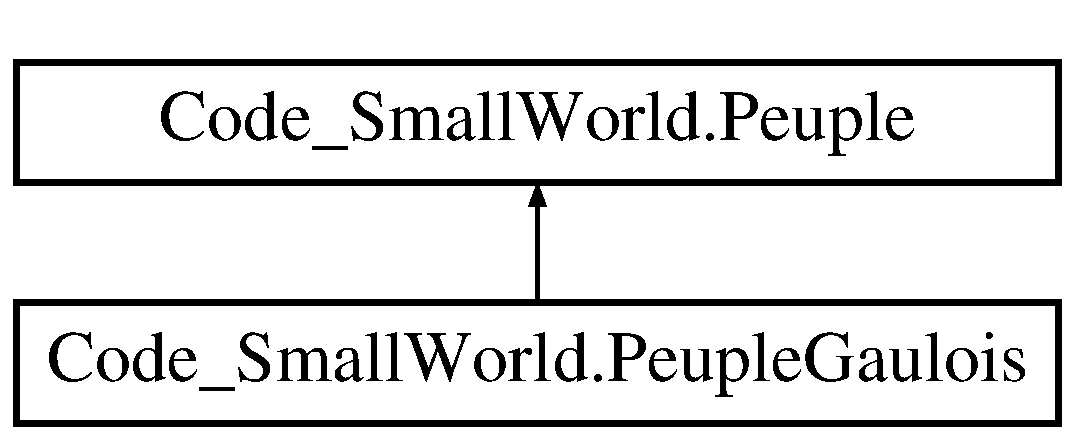
\includegraphics[height=2.000000cm]{interface_code___small_world_1_1_peuple_gaulois}
\end{center}
\end{figure}
\subsection*{Additional Inherited Members}


The documentation for this interface was generated from the following file\-:\begin{DoxyCompactItemize}
\item 
C\-:/\-Users/damienc/\-Documents/\-Git\-Hub/\-Small\-World/\-Visual\-Studio/\-Projet\-P\-O\-O/Peuple\-Gaulois.\-cs\end{DoxyCompactItemize}

\hypertarget{interface_code___small_world_1_1_peuple_nain}{\section{Code\-\_\-\-Small\-World.\-Peuple\-Nain Interface Reference}
\label{interface_code___small_world_1_1_peuple_nain}\index{Code\-\_\-\-Small\-World.\-Peuple\-Nain@{Code\-\_\-\-Small\-World.\-Peuple\-Nain}}
}
Inheritance diagram for Code\-\_\-\-Small\-World.\-Peuple\-Nain\-:\begin{figure}[H]
\begin{center}
\leavevmode
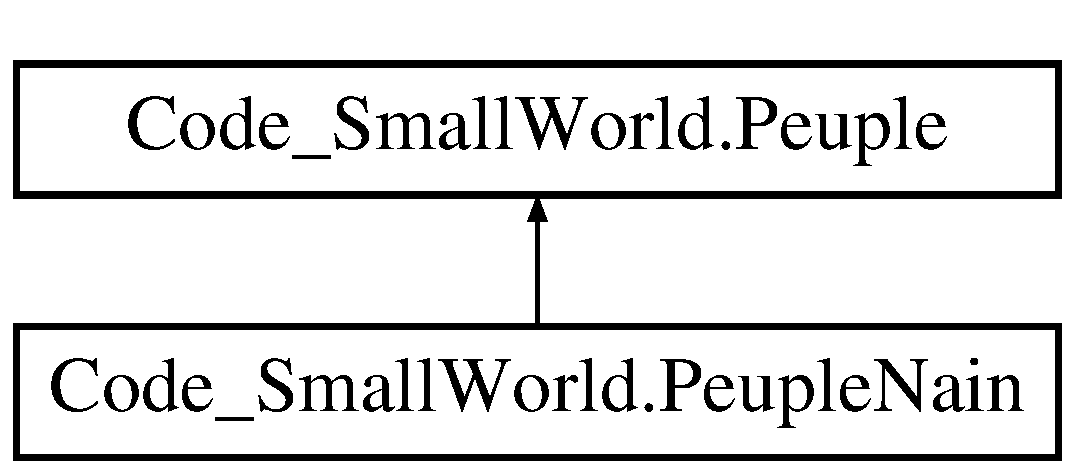
\includegraphics[height=2.000000cm]{interface_code___small_world_1_1_peuple_nain}
\end{center}
\end{figure}
\subsection*{Additional Inherited Members}


The documentation for this interface was generated from the following file\-:\begin{DoxyCompactItemize}
\item 
C\-:/\-Users/damienc/\-Documents/\-Git\-Hub/\-Small\-World/\-Visual\-Studio/\-Projet\-P\-O\-O/Peuple\-Nain.\-cs\end{DoxyCompactItemize}

\hypertarget{interface_code___small_world_1_1_peuple_viking}{\section{Code\-\_\-\-Small\-World.\-Peuple\-Viking Interface Reference}
\label{interface_code___small_world_1_1_peuple_viking}\index{Code\-\_\-\-Small\-World.\-Peuple\-Viking@{Code\-\_\-\-Small\-World.\-Peuple\-Viking}}
}
Inheritance diagram for Code\-\_\-\-Small\-World.\-Peuple\-Viking\-:\begin{figure}[H]
\begin{center}
\leavevmode
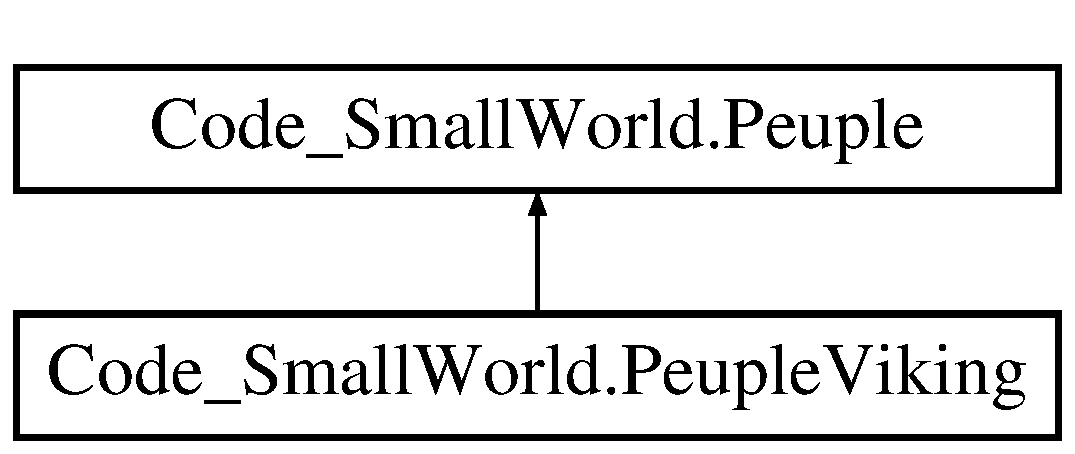
\includegraphics[height=2.000000cm]{interface_code___small_world_1_1_peuple_viking}
\end{center}
\end{figure}
\subsection*{Additional Inherited Members}


The documentation for this interface was generated from the following file\-:\begin{DoxyCompactItemize}
\item 
C\-:/\-Users/damienc/\-Documents/\-Git\-Hub/\-Small\-World/\-Visual\-Studio/\-Projet\-P\-O\-O/Peuple\-Viking.\-cs\end{DoxyCompactItemize}

\hypertarget{interface_code___small_world_1_1_plaine}{\section{Code\-\_\-\-Small\-World.\-Plaine Interface Reference}
\label{interface_code___small_world_1_1_plaine}\index{Code\-\_\-\-Small\-World.\-Plaine@{Code\-\_\-\-Small\-World.\-Plaine}}
}
Inheritance diagram for Code\-\_\-\-Small\-World.\-Plaine\-:\begin{figure}[H]
\begin{center}
\leavevmode
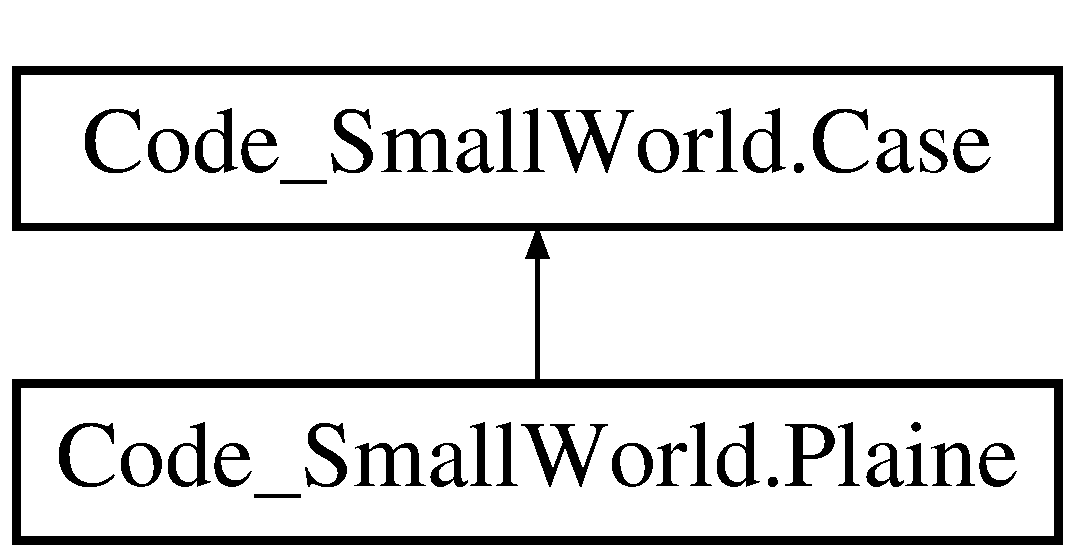
\includegraphics[height=2.000000cm]{interface_code___small_world_1_1_plaine}
\end{center}
\end{figure}


The documentation for this interface was generated from the following file\-:\begin{DoxyCompactItemize}
\item 
C\-:/\-Users/damienc/\-Documents/\-Git\-Hub/\-Small\-World/\-Visual\-Studio/\-Projet\-P\-O\-O/plaine.\-cs\end{DoxyCompactItemize}

\hypertarget{interface_code___small_world_1_1_sauvegarde}{\section{Code\-\_\-\-Small\-World.\-Sauvegarde Interface Reference}
\label{interface_code___small_world_1_1_sauvegarde}\index{Code\-\_\-\-Small\-World.\-Sauvegarde@{Code\-\_\-\-Small\-World.\-Sauvegarde}}
}
\subsection*{Public Member Functions}
\begin{DoxyCompactItemize}
\item 
\hypertarget{interface_code___small_world_1_1_sauvegarde_aa42959c5c48617c7ec92761073dd3c9c}{void {\bfseries charge} ()}\label{interface_code___small_world_1_1_sauvegarde_aa42959c5c48617c7ec92761073dd3c9c}

\item 
\hypertarget{interface_code___small_world_1_1_sauvegarde_aae150a11c73d425342b1592eaf71c9ff}{void {\bfseries enregistrer} ()}\label{interface_code___small_world_1_1_sauvegarde_aae150a11c73d425342b1592eaf71c9ff}

\end{DoxyCompactItemize}


The documentation for this interface was generated from the following file\-:\begin{DoxyCompactItemize}
\item 
C\-:/\-Users/damienc/\-Documents/\-Git\-Hub/\-Small\-World/\-Visual\-Studio/\-Projet\-P\-O\-O/Sauvegarder.\-cs\end{DoxyCompactItemize}

\hypertarget{interface_code___small_world_1_1_strategie_carte}{\section{Code\-\_\-\-Small\-World.\-Strategie\-Carte Interface Reference}
\label{interface_code___small_world_1_1_strategie_carte}\index{Code\-\_\-\-Small\-World.\-Strategie\-Carte@{Code\-\_\-\-Small\-World.\-Strategie\-Carte}}
}
Inheritance diagram for Code\-\_\-\-Small\-World.\-Strategie\-Carte\-:\begin{figure}[H]
\begin{center}
\leavevmode
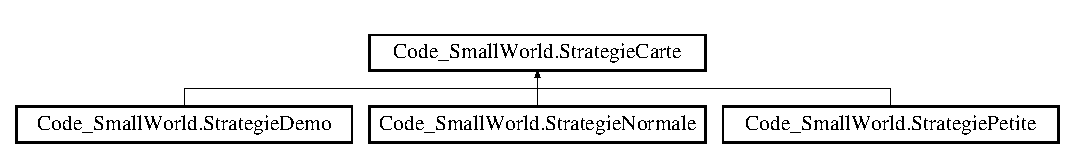
\includegraphics[height=1.689291cm]{interface_code___small_world_1_1_strategie_carte}
\end{center}
\end{figure}
\subsection*{Public Member Functions}
\begin{DoxyCompactItemize}
\item 
void \hyperlink{interface_code___small_world_1_1_strategie_carte_a0d74960263e0d6c0abc3c4f5802d9f29}{construire} ()
\end{DoxyCompactItemize}


\subsection{Member Function Documentation}
\hypertarget{interface_code___small_world_1_1_strategie_carte_a0d74960263e0d6c0abc3c4f5802d9f29}{\index{Code\-\_\-\-Small\-World\-::\-Strategie\-Carte@{Code\-\_\-\-Small\-World\-::\-Strategie\-Carte}!construire@{construire}}
\index{construire@{construire}!Code_SmallWorld::StrategieCarte@{Code\-\_\-\-Small\-World\-::\-Strategie\-Carte}}
\subsubsection[{construire}]{\setlength{\rightskip}{0pt plus 5cm}void Code\-\_\-\-Small\-World.\-Strategie\-Carte.\-construire (
\begin{DoxyParamCaption}
{}
\end{DoxyParamCaption}
)}}\label{interface_code___small_world_1_1_strategie_carte_a0d74960263e0d6c0abc3c4f5802d9f29}


Implemented in \hyperlink{interface_code___small_world_1_1_strategie_demo_ad1a9a92e328a5e7f5ec14e38ba7d1833}{Code\-\_\-\-Small\-World.\-Strategie\-Demo}, \hyperlink{interface_code___small_world_1_1_strategie_normale_aecfd7030a93351fdb1a8403b52cbd771}{Code\-\_\-\-Small\-World.\-Strategie\-Normale}, and \hyperlink{interface_code___small_world_1_1_strategie_petite_ac163c0ea76fbcf616f93aa28dbc3bdc6}{Code\-\_\-\-Small\-World.\-Strategie\-Petite}.



The documentation for this interface was generated from the following file\-:\begin{DoxyCompactItemize}
\item 
C\-:/\-Users/damienc/\-Documents/\-Git\-Hub/\-Small\-World/\-Visual\-Studio/\-Projet\-P\-O\-O/Carte.\-cs\end{DoxyCompactItemize}

\hypertarget{interface_code___small_world_1_1_strategie_demo}{\section{Code\-\_\-\-Small\-World.\-Strategie\-Demo Interface Reference}
\label{interface_code___small_world_1_1_strategie_demo}\index{Code\-\_\-\-Small\-World.\-Strategie\-Demo@{Code\-\_\-\-Small\-World.\-Strategie\-Demo}}
}
Inheritance diagram for Code\-\_\-\-Small\-World.\-Strategie\-Demo\-:\begin{figure}[H]
\begin{center}
\leavevmode
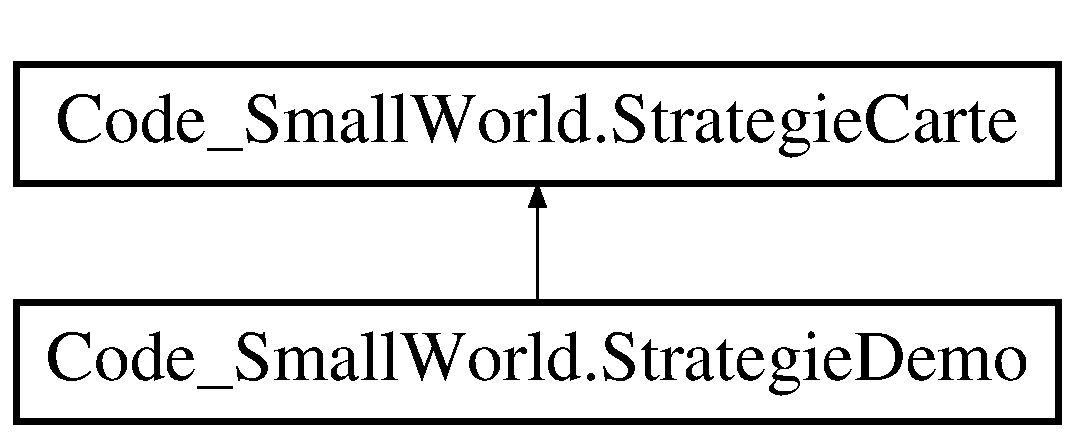
\includegraphics[height=2.000000cm]{interface_code___small_world_1_1_strategie_demo}
\end{center}
\end{figure}
\subsection*{Public Member Functions}
\begin{DoxyCompactItemize}
\item 
void \hyperlink{interface_code___small_world_1_1_strategie_demo_ad1a9a92e328a5e7f5ec14e38ba7d1833}{construire} ()
\end{DoxyCompactItemize}


\subsection{Member Function Documentation}
\hypertarget{interface_code___small_world_1_1_strategie_demo_ad1a9a92e328a5e7f5ec14e38ba7d1833}{\index{Code\-\_\-\-Small\-World\-::\-Strategie\-Demo@{Code\-\_\-\-Small\-World\-::\-Strategie\-Demo}!construire@{construire}}
\index{construire@{construire}!Code_SmallWorld::StrategieDemo@{Code\-\_\-\-Small\-World\-::\-Strategie\-Demo}}
\subsubsection[{construire}]{\setlength{\rightskip}{0pt plus 5cm}void Code\-\_\-\-Small\-World.\-Strategie\-Demo.\-construire (
\begin{DoxyParamCaption}
{}
\end{DoxyParamCaption}
)}}\label{interface_code___small_world_1_1_strategie_demo_ad1a9a92e328a5e7f5ec14e38ba7d1833}


Implements \hyperlink{interface_code___small_world_1_1_strategie_carte_a0d74960263e0d6c0abc3c4f5802d9f29}{Code\-\_\-\-Small\-World.\-Strategie\-Carte}.



The documentation for this interface was generated from the following file\-:\begin{DoxyCompactItemize}
\item 
C\-:/\-Users/damienc/\-Documents/\-Git\-Hub/\-Small\-World/\-Visual\-Studio/\-Projet\-P\-O\-O/Demo.\-cs\end{DoxyCompactItemize}

\hypertarget{interface_code___small_world_1_1_strategie_normale}{\section{Code\-\_\-\-Small\-World.\-Strategie\-Normale Interface Reference}
\label{interface_code___small_world_1_1_strategie_normale}\index{Code\-\_\-\-Small\-World.\-Strategie\-Normale@{Code\-\_\-\-Small\-World.\-Strategie\-Normale}}
}
Inheritance diagram for Code\-\_\-\-Small\-World.\-Strategie\-Normale\-:\begin{figure}[H]
\begin{center}
\leavevmode
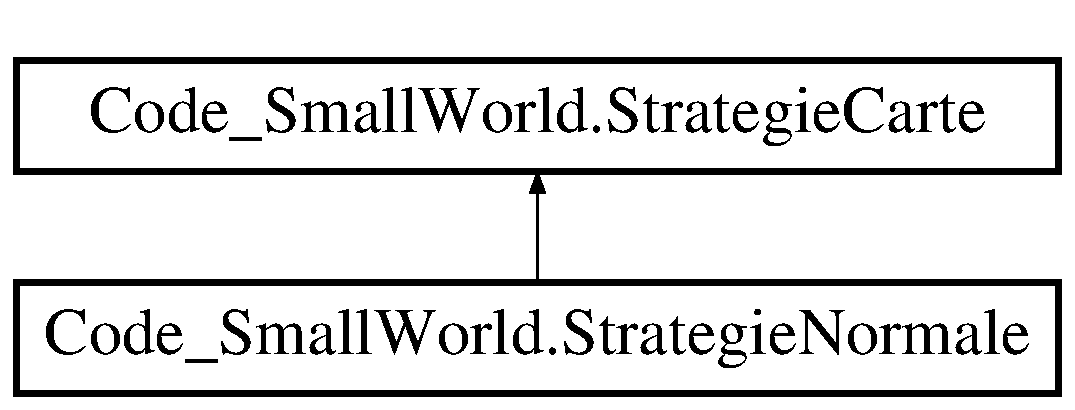
\includegraphics[height=2.000000cm]{interface_code___small_world_1_1_strategie_normale}
\end{center}
\end{figure}
\subsection*{Public Member Functions}
\begin{DoxyCompactItemize}
\item 
void \hyperlink{interface_code___small_world_1_1_strategie_normale_aecfd7030a93351fdb1a8403b52cbd771}{construire} ()
\end{DoxyCompactItemize}


\subsection{Member Function Documentation}
\hypertarget{interface_code___small_world_1_1_strategie_normale_aecfd7030a93351fdb1a8403b52cbd771}{\index{Code\-\_\-\-Small\-World\-::\-Strategie\-Normale@{Code\-\_\-\-Small\-World\-::\-Strategie\-Normale}!construire@{construire}}
\index{construire@{construire}!Code_SmallWorld::StrategieNormale@{Code\-\_\-\-Small\-World\-::\-Strategie\-Normale}}
\subsubsection[{construire}]{\setlength{\rightskip}{0pt plus 5cm}void Code\-\_\-\-Small\-World.\-Strategie\-Normale.\-construire (
\begin{DoxyParamCaption}
{}
\end{DoxyParamCaption}
)}}\label{interface_code___small_world_1_1_strategie_normale_aecfd7030a93351fdb1a8403b52cbd771}


Implements \hyperlink{interface_code___small_world_1_1_strategie_carte_a0d74960263e0d6c0abc3c4f5802d9f29}{Code\-\_\-\-Small\-World.\-Strategie\-Carte}.



The documentation for this interface was generated from the following file\-:\begin{DoxyCompactItemize}
\item 
C\-:/\-Users/damienc/\-Documents/\-Git\-Hub/\-Small\-World/\-Visual\-Studio/\-Projet\-P\-O\-O/Normale.\-cs\end{DoxyCompactItemize}

\hypertarget{interface_code___small_world_1_1_strategie_petite}{\section{Code\-\_\-\-Small\-World.\-Strategie\-Petite Interface Reference}
\label{interface_code___small_world_1_1_strategie_petite}\index{Code\-\_\-\-Small\-World.\-Strategie\-Petite@{Code\-\_\-\-Small\-World.\-Strategie\-Petite}}
}
Inheritance diagram for Code\-\_\-\-Small\-World.\-Strategie\-Petite\-:\begin{figure}[H]
\begin{center}
\leavevmode
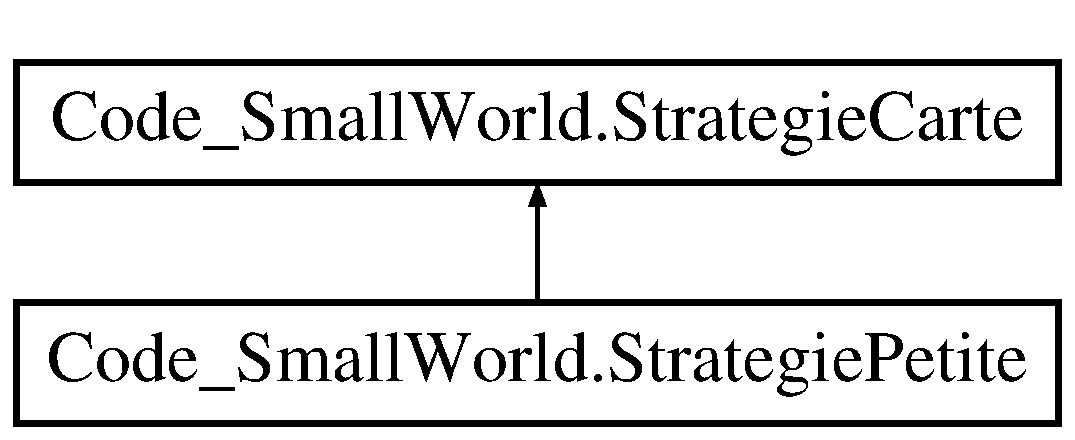
\includegraphics[height=2.000000cm]{interface_code___small_world_1_1_strategie_petite}
\end{center}
\end{figure}
\subsection*{Public Member Functions}
\begin{DoxyCompactItemize}
\item 
void \hyperlink{interface_code___small_world_1_1_strategie_petite_ac163c0ea76fbcf616f93aa28dbc3bdc6}{construire} ()
\end{DoxyCompactItemize}


\subsection{Member Function Documentation}
\hypertarget{interface_code___small_world_1_1_strategie_petite_ac163c0ea76fbcf616f93aa28dbc3bdc6}{\index{Code\-\_\-\-Small\-World\-::\-Strategie\-Petite@{Code\-\_\-\-Small\-World\-::\-Strategie\-Petite}!construire@{construire}}
\index{construire@{construire}!Code_SmallWorld::StrategiePetite@{Code\-\_\-\-Small\-World\-::\-Strategie\-Petite}}
\subsubsection[{construire}]{\setlength{\rightskip}{0pt plus 5cm}void Code\-\_\-\-Small\-World.\-Strategie\-Petite.\-construire (
\begin{DoxyParamCaption}
{}
\end{DoxyParamCaption}
)}}\label{interface_code___small_world_1_1_strategie_petite_ac163c0ea76fbcf616f93aa28dbc3bdc6}


Implements \hyperlink{interface_code___small_world_1_1_strategie_carte_a0d74960263e0d6c0abc3c4f5802d9f29}{Code\-\_\-\-Small\-World.\-Strategie\-Carte}.



The documentation for this interface was generated from the following file\-:\begin{DoxyCompactItemize}
\item 
C\-:/\-Users/damienc/\-Documents/\-Git\-Hub/\-Small\-World/\-Visual\-Studio/\-Projet\-P\-O\-O/Petite.\-cs\end{DoxyCompactItemize}

\hypertarget{interface_code___small_world_1_1_unite}{\section{Code\-\_\-\-Small\-World.\-Unite Interface Reference}
\label{interface_code___small_world_1_1_unite}\index{Code\-\_\-\-Small\-World.\-Unite@{Code\-\_\-\-Small\-World.\-Unite}}
}
Inheritance diagram for Code\-\_\-\-Small\-World.\-Unite\-:\begin{figure}[H]
\begin{center}
\leavevmode
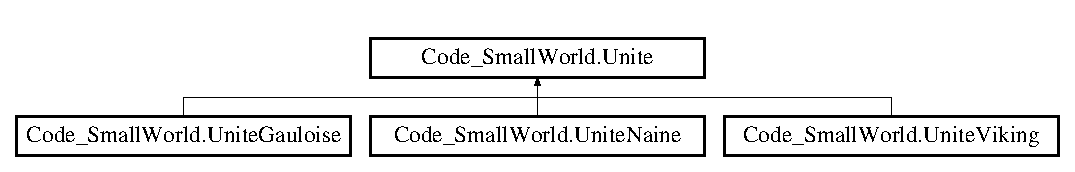
\includegraphics[height=1.857380cm]{interface_code___small_world_1_1_unite}
\end{center}
\end{figure}
\subsection*{Public Member Functions}
\begin{DoxyCompactItemize}
\item 
\hypertarget{interface_code___small_world_1_1_unite_aca6d6724bda323a6d38b28f910e500aa}{void {\bfseries attaquer} ()}\label{interface_code___small_world_1_1_unite_aca6d6724bda323a6d38b28f910e500aa}

\item 
\hypertarget{interface_code___small_world_1_1_unite_ab2bcb3c1c951a555f72d48e7e554a125}{void {\bfseries deplacer} ()}\label{interface_code___small_world_1_1_unite_ab2bcb3c1c951a555f72d48e7e554a125}

\end{DoxyCompactItemize}


The documentation for this interface was generated from the following file\-:\begin{DoxyCompactItemize}
\item 
C\-:/\-Users/damienc/\-Documents/\-Git\-Hub/\-Small\-World/\-Visual\-Studio/\-Projet\-P\-O\-O/Unite.\-cs\end{DoxyCompactItemize}

\hypertarget{interface_code___small_world_1_1_unite_gauloise}{\section{Code\-\_\-\-Small\-World.\-Unite\-Gauloise Interface Reference}
\label{interface_code___small_world_1_1_unite_gauloise}\index{Code\-\_\-\-Small\-World.\-Unite\-Gauloise@{Code\-\_\-\-Small\-World.\-Unite\-Gauloise}}
}
Inheritance diagram for Code\-\_\-\-Small\-World.\-Unite\-Gauloise\-:\begin{figure}[H]
\begin{center}
\leavevmode
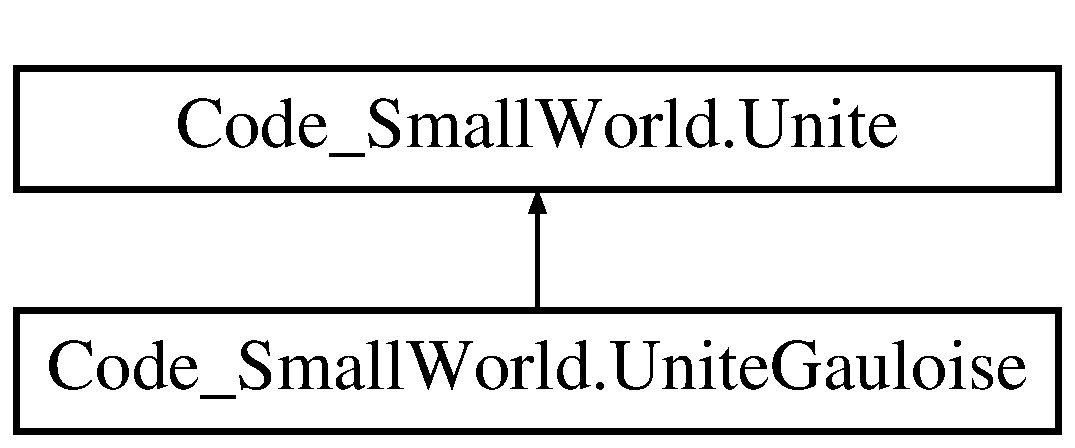
\includegraphics[height=2.000000cm]{interface_code___small_world_1_1_unite_gauloise}
\end{center}
\end{figure}
\subsection*{Additional Inherited Members}


The documentation for this interface was generated from the following file\-:\begin{DoxyCompactItemize}
\item 
C\-:/\-Users/damienc/\-Documents/\-Git\-Hub/\-Small\-World/\-Visual\-Studio/\-Projet\-P\-O\-O/Unite\-Gauloise.\-cs\end{DoxyCompactItemize}

\hypertarget{interface_code___small_world_1_1_unite_naine}{\section{Code\-\_\-\-Small\-World.\-Unite\-Naine Interface Reference}
\label{interface_code___small_world_1_1_unite_naine}\index{Code\-\_\-\-Small\-World.\-Unite\-Naine@{Code\-\_\-\-Small\-World.\-Unite\-Naine}}
}
Inheritance diagram for Code\-\_\-\-Small\-World.\-Unite\-Naine\-:\begin{figure}[H]
\begin{center}
\leavevmode
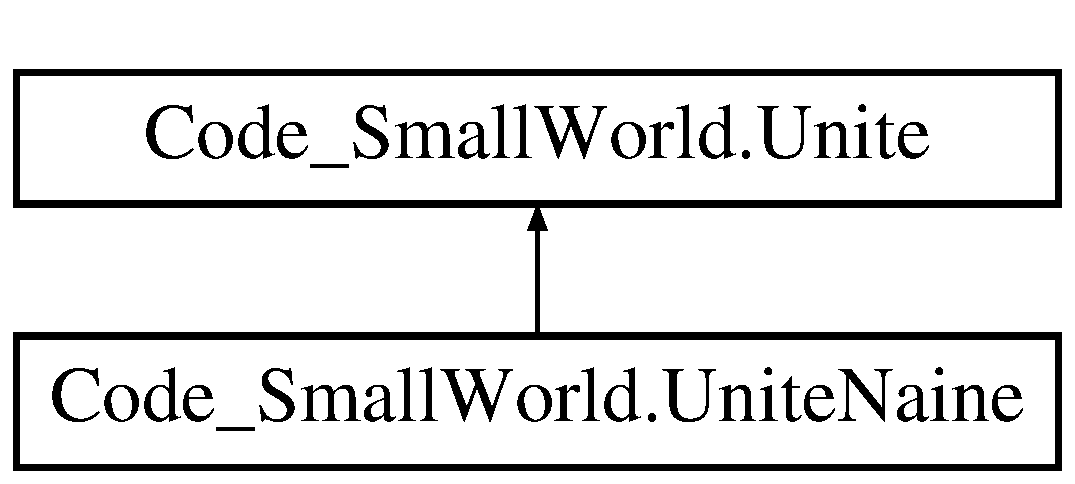
\includegraphics[height=2.000000cm]{interface_code___small_world_1_1_unite_naine}
\end{center}
\end{figure}
\subsection*{Additional Inherited Members}


The documentation for this interface was generated from the following file\-:\begin{DoxyCompactItemize}
\item 
C\-:/\-Users/damienc/\-Documents/\-Git\-Hub/\-Small\-World/\-Visual\-Studio/\-Projet\-P\-O\-O/Unite\-Naine.\-cs\end{DoxyCompactItemize}

\hypertarget{interface_code___small_world_1_1_unite_viking}{\section{Code\-\_\-\-Small\-World.\-Unite\-Viking Interface Reference}
\label{interface_code___small_world_1_1_unite_viking}\index{Code\-\_\-\-Small\-World.\-Unite\-Viking@{Code\-\_\-\-Small\-World.\-Unite\-Viking}}
}
Inheritance diagram for Code\-\_\-\-Small\-World.\-Unite\-Viking\-:\begin{figure}[H]
\begin{center}
\leavevmode
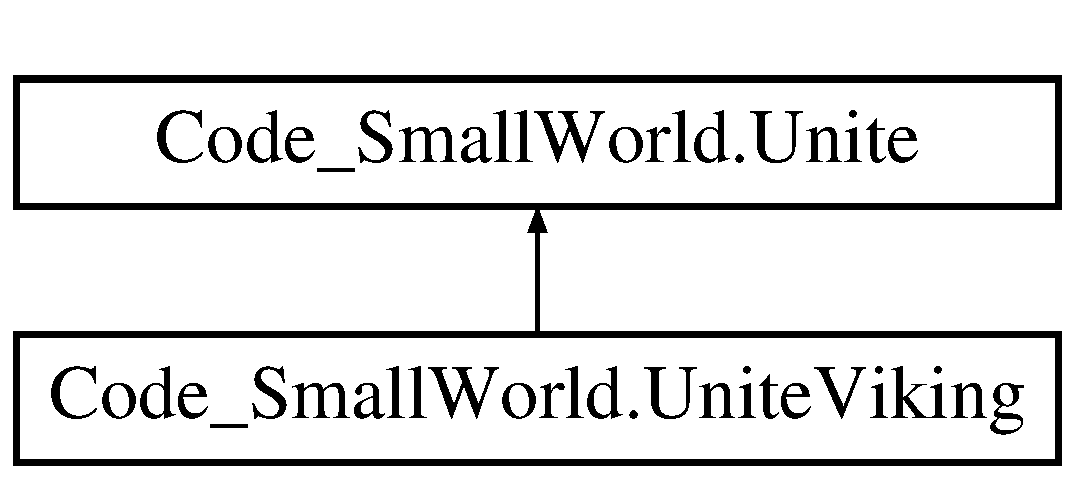
\includegraphics[height=2.000000cm]{interface_code___small_world_1_1_unite_viking}
\end{center}
\end{figure}
\subsection*{Additional Inherited Members}


The documentation for this interface was generated from the following file\-:\begin{DoxyCompactItemize}
\item 
C\-:/\-Users/damienc/\-Documents/\-Git\-Hub/\-Small\-World/\-Visual\-Studio/\-Projet\-P\-O\-O/Unite\-Viking.\-cs\end{DoxyCompactItemize}

\hypertarget{interface_code___small_world_1_1_viking}{\section{Code\-\_\-\-Small\-World.\-Viking Interface Reference}
\label{interface_code___small_world_1_1_viking}\index{Code\-\_\-\-Small\-World.\-Viking@{Code\-\_\-\-Small\-World.\-Viking}}
}


The documentation for this interface was generated from the following file\-:\begin{DoxyCompactItemize}
\item 
C\-:/\-Users/damienc/\-Documents/\-Git\-Hub/\-Small\-World/\-Visual\-Studio/\-Projet\-P\-O\-O/Viking.\-cs\end{DoxyCompactItemize}

%--- End generated contents ---

% Index
\newpage
\phantomsection
\addcontentsline{toc}{part}{Index}
\printindex

\end{document}
